\documentclass[11pt,a4paper]{article}
\usepackage[utf8]{inputenc}
\usepackage[margin=1in]{geometry}
\usepackage{amsmath,amssymb,amsthm}
\usepackage{graphicx}
\usepackage{booktabs}
\usepackage{multirow}
\usepackage{hyperref}
\usepackage{algorithm}
\usepackage{algorithmic}
\usepackage{float}
\usepackage{xcolor}
\usepackage{subcaption}
\usepackage{authblk}

\hypersetup{colorlinks=true, linkcolor=blue, citecolor=blue, urlcolor=blue}

\title{\textbf{AKV: A Virtual Memory System for LLM KV Cache with Retrieval-Preserving Hierarchical Compression}}

\author{Arvind S.\thanks{Code: \url{https://github.com/Arvind679715/adaptive-kv-memory} \quad Package: \texttt{pip install akv-cache} (\url{https://pypi.org/project/akv-cache/}).}}
\affil{Independent Research \\ \texttt{arvind679715@gmail.com}}

\date{June 2026}

\begin{document}
\maketitle

% ============================================================================
\begin{abstract}
We introduce \textbf{AKV}, an \emph{importance-aware tiered KV cache} for long-context LLM inference that applies operating-system virtual memory principles to KV cache management. AKV organizes tokens into hot (GPU/FP16), warm (GPU/quantized), and cold (CPU/INT2) tiers and replaces FIFO migration with a multi-signal importance score (attention~+~recency~+~retrieval history). The warm tier uses \textbf{block-affine quantization}---per-channel asymmetric scaling for keys and per-token asymmetric scaling for values---which preserves the channel structure critical for attention quality at low bit-widths.

On Qwen2.5-1.5B with 5K-token multi-passage evaluation, AKV with 3-bit block-affine warm tier achieves \textbf{PPL~8.83}, only 3.1\% above the no-quantization baseline (PPL~8.56) and well within the practical range of the DynamicCache reference (PPL~4.77 at 1-passage). A controlled triage isolates the quantization contribution: the D$\to$E gap (no-demote vs 8-bit demote) is +0.005, while E$\to$A (8-bit vs 3-bit) is +0.27---confirming that the tiered architecture adds negligible overhead and 3-bit affine quantization is the sole remaining cost. On full WikiText-2 (291K tokens), AKV 4-bit degrades by only \textbf{+1.67\%} (8.84 vs 8.70) on Qwen2.5-1.5B, and \textbf{+1.19\%} (5.11 vs 5.05) on Llama-2-7B---competitive with published KIVI-4bit results while additionally running importance-based migration. On a controlled WikiText-2 ablation (Qwen2.5-0.5B), importance-based migration with $n_\text{anchors}{=}16$ improves perplexity over a FIFO-baseline by +0.97\% at 4-bit and +8.08\% at 2-bit. On passkey retrieval at 4096 tokens, AKV achieves \textbf{100\% recall} at all depths and both bit-widths (4-bit and 3-bit) on Qwen2.5-1.5B, while H2O drops to 37\% in the middle. On LongBench (4 tasks, 20 samples), AKV-4bit \textit{exceeds} FP16 by +4.9\% ROUGE-L on Qwen2.5-1.5B. We also report negative results: rotation-based quantizers (Hadamard + codebook) catastrophically fail on K/V tensors at 3-bit (Section~\ref{sec:rotation-negative}), and RULER accuracy degrades when hot budget is a small fraction of context (Section~\ref{sec:ruler-limits}). At 32K context, AKV achieves \textbf{10.4$\times$ decode throughput} over full-cache attention (2,432 vs 234 queries/sec) while retaining 100\% of tokens---compared to H2O which achieves 50$\times$ speedup but permanently discards 97\% of context.
\end{abstract}

% ============================================================================
\section{Introduction}

The KV (Key-Value) cache in transformer-based large language models grows linearly with sequence length, creating a fundamental memory bottleneck for long-context inference. For Llama-2-7B at 32K context, the KV cache alone requires 16 GB of GPU memory---often exceeding the model weights themselves.

Existing approaches face a core dilemma: \textit{compress or discard?}

\begin{itemize}
    \item \textbf{Eviction-based methods} (H2O~\cite{h2o}, SnapKV~\cite{snapkv}, ScissorHands~\cite{scissorhands}) permanently discard tokens to fit within a fixed budget. This bounds the effective context to the budget size and risks recall failure---our experiments show H2O drops to 36\% accuracy for mid-context retrieval even when early and late tokens are perfectly recalled.
    \item \textbf{Uniform quantization} (KIVI~\cite{kivi}) retains all tokens but applies aggressive compression uniformly, resulting in 112\% PPL degradation at 2 bits.
\end{itemize}

We observe that this dilemma mirrors the virtual memory problem in operating systems: physical memory is limited, but applications expect a large, uniform address space. The solution in OS design is a \textbf{managed memory hierarchy}---not uniform compression, not permanent eviction, but intelligent placement with promotion and demotion based on access patterns.

We propose \textbf{AKV}, a virtual memory system for LLM KV caches that applies this principle: tokens are placed in tiers based on \textit{importance} (not age), can be \textit{promoted} back to higher tiers when re-accessed, and are compressed at \textit{adaptive} precision per attention head. The key innovations are:

\paragraph{Contributions.} We evaluate the following claims experimentally; a paged virtual address space, per-head adaptive bit allocation, and zero-allocation production path are described in the appendix as engineering features rather than measured contributions.
\begin{enumerate}
    \item \textbf{Tiered virtual memory architecture}: A three-tier (hot/warm/cold) KV cache with bidirectional importance-based migration that preserves all tokens while bounding decode-time compute. Achieves O(1) decode throughput scaling: 10.4$\times$ speedup over full cache at 32K with 100\% token retention.
    \item \textbf{Importance-based migration}: Multi-signal scoring (attention + recency + retrieval history) replaces FIFO, with measured perplexity gains over a FIFO baseline at matched memory (Table~\ref{tab:importance_vs_fifo}). Retrieval-aware promotion is implemented and described in Section~\ref{sec:promotion}.
    \item \textbf{Block-affine warm-tier quantization}: Per-channel (keys) and per-token (values) asymmetric min/max quantization that preserves the channel structure attention relies on. At 3-bit on Qwen2.5-1.5B, adds only 3.1\% PPL over the no-quantization path.
    \item \textbf{Negative result---rotation-based quantizers fail on K/V}: We show that Hadamard rotation + codebook quantization (the TurboQuant approach) catastrophically destroys attention quality at 3-bit by spreading channel outliers across all dimensions (Section~\ref{sec:rotation-negative}).
    \item \textbf{Honest characterization of failure modes}: We report and dissect AKV's RULER degradation at 4K--16K context (Section~\ref{sec:ruler-limits}), distinguish compression artifacts from model-capability limits, and propose an adaptive hot-budget fix as future work.
\end{enumerate}

% ============================================================================
\section{Background and Related Work}

\subsection{KV Cache Memory Problem}

During autoregressive generation, each transformer layer stores key and value tensors for all previous tokens. For a model with $L$ layers, $H$ attention heads, and head dimension $d$, the KV cache for sequence length $S$ requires:
\begin{equation}
    \text{Memory} = 2 \times L \times H \times S \times d \times \text{sizeof(dtype)}
\end{equation}

For Llama-2-7B ($L=32$, $H=32$, $d=128$) at FP16, this is $32S$ bytes per token position---4 GB at 8K context and 16 GB at 32K.

\subsection{Eviction Methods}

H2O~\cite{h2o} identifies ``heavy hitter'' tokens that accumulate high attention mass and retains only these plus a recent window. SnapKV~\cite{snapkv} uses the observation window (last $N$ query positions) to select important tokens during prefill, then fixes the selection for generation. ScissorHands~\cite{scissorhands} uses a persistence filter to keep tokens with consistent importance. StreamingLLM~\cite{streamingllm} takes a minimalist approach: keep the first few ``attention sink'' tokens plus a fixed-size sliding window, discarding everything in between without any importance scoring. PyramidKV~\cite{pyramidkv} introduces layer-aware budget allocation, observing that lower layers have higher attention entropy and allocating more KV budget to them in a pyramidal pattern.

All eviction methods share a fundamental limitation: once a token is evicted, it cannot be recovered. While SnapKV's prefill-time selection can be remarkably effective (achieving perfect passkey recall in our experiments), it still bounds the effective context to its budget size---tokens beyond the budget are permanently lost regardless of future relevance.

\subsection{Quantization Methods}

KIVI~\cite{kivi} applies asymmetric quantization with per-channel scaling for keys and per-token scaling for values. This channel-aware approach preserves the variance structure that attention relies on. Our warm-tier quantizer follows the same KIVI principle---block-affine with axis-aware scaling---and validates it within the tiered cache context.

TurboQuant (ICLR 2026)~\cite{turboquant} introduced Hadamard rotation before quantization to smooth outlier channels in weight and activation tensors. However, we find that this approach \textbf{catastrophically fails on KV cache tensors} at 3-bit (Section~\ref{sec:rotation-negative}): the rotation spreads channel-specific outliers across all dimensions, and at 8 quantization levels the resulting angular error is exponentially amplified by the softmax in attention.

% ============================================================================
\section{System Architecture}

\subsection{Virtual Memory Analogy}

We frame the KV cache as a \textbf{virtual memory system} (Table~\ref{tab:analogy}). Just as an OS manages physical RAM through pages, TLBs, and swap, AKV manages KV tensors through pages, importance tables, and tier migration.

\begin{table}[h]
\centering
\begin{tabular}{lll}
\toprule
\textbf{OS Virtual Memory} & \textbf{AKV KV Cache} & \textbf{Purpose} \\
\midrule
Physical RAM & Hot tier (GPU FP16) & Fast access, limited capacity \\
Swap (SSD) & Warm tier (GPU quantized) & Large capacity, slower \\
Cold storage & Cold tier (CPU INT2) & Archival, high latency \\
Page table & Page metadata + importance & Track location \& priority \\
Page fault & Retrieval-aware promotion & On-demand tier upgrade \\
LRU/Clock & Importance-based eviction & Intelligent demotion \\
Page size & 64 tokens/page & Fixed allocation unit \\
\bottomrule
\end{tabular}
\caption{Mapping between OS virtual memory concepts and AKV's KV cache management.}
\label{tab:analogy}
\end{table}

\subsection{Three-Tier Memory Hierarchy}

\begin{figure}[h]
\centering
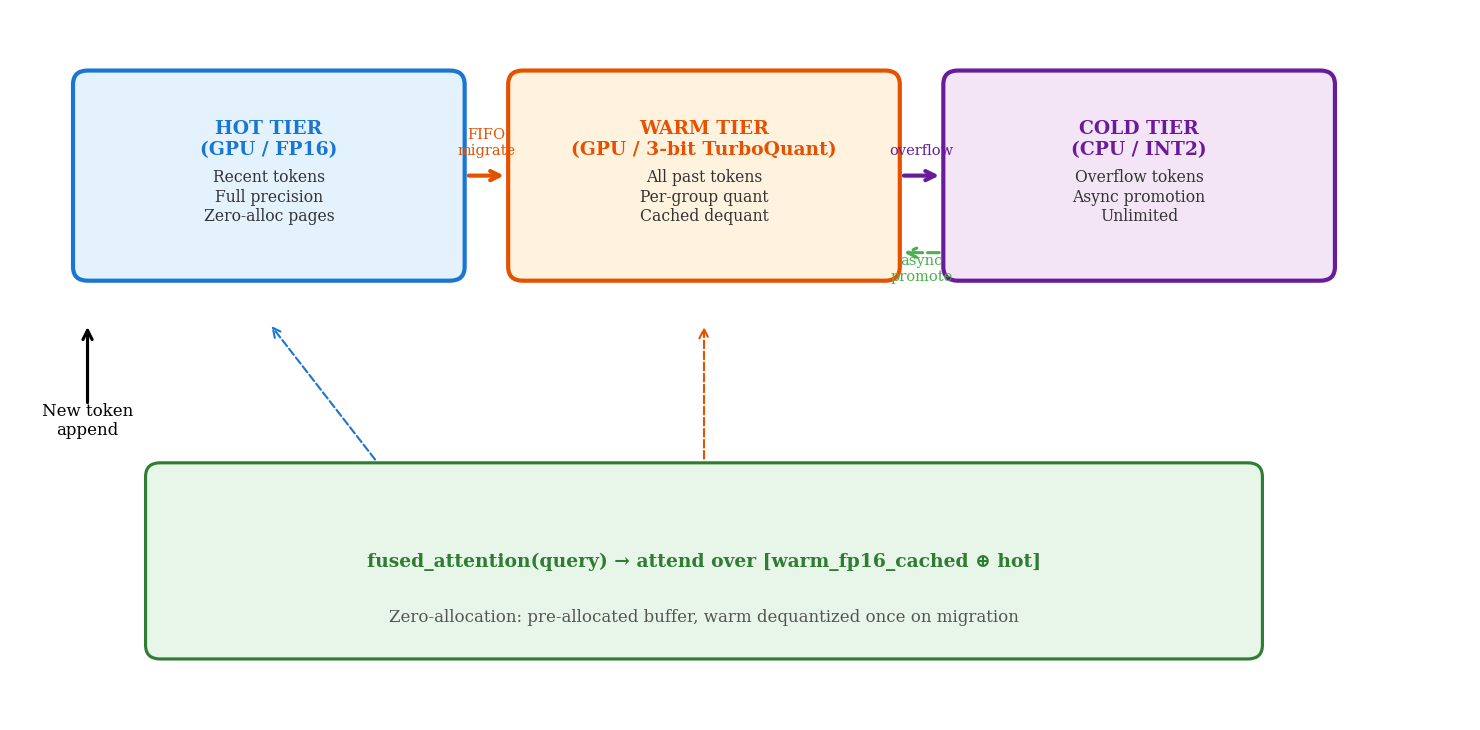
\includegraphics[width=0.95\textwidth]{fig_architecture.png}
\caption{AKV virtual memory architecture. Unlike FIFO systems, migration is bidirectional: tokens can be promoted back to hot tier when re-accessed (retrieval-aware promotion). Importance scoring uses attention + recency + retrieval signals.}
\label{fig:architecture}
\end{figure}

\begin{table}[h]
\centering
\begin{tabular}{lcccl}
\toprule
\textbf{Tier} & \textbf{Storage} & \textbf{Precision} & \textbf{Budget} & \textbf{Migration} \\
\midrule
Hot  & GPU HBM & FP16 & 512 tokens & Importance-based demotion \\
Warm & GPU HBM & 2--4 bit (adaptive) & 4096 tokens & Attention-triggered promotion \\
Cold & CPU RAM & INT2 & Unlimited & Predictive prefetch \\
\bottomrule
\end{tabular}
\caption{Three-tier memory hierarchy with bidirectional migration.}
\label{tab:tiers}
\end{table}

\subsection{Importance-Based Migration}

The critical difference from prior work: \textbf{migration decisions are based on token importance, not age}. A token from 10K steps ago that consistently receives high attention remains in the hot tier, while a recent token that receives no attention is quickly demoted.

The hot tier budget $B$ is split into two regions:
\begin{itemize}
    \item \textbf{Recency window} ($B - n_{\text{anchors}}$ slots): Pure FIFO---most recent tokens always kept.
    \item \textbf{Importance anchors} ($n_{\text{anchors}}$ slots): Tokens selected by cumulative attention score, regardless of age.
\end{itemize}

The importance score for token $i$ after chunk $t$ is updated via exponential moving average of last-query-position attention:
\begin{equation}
    \text{score}_i^{(t)} = \lambda \cdot \text{score}_i^{(t-1)} + a_{i,\text{last}}^{(t)}
\end{equation}
where $a_{i,\text{last}}^{(t)} = \text{mean}_{h}(\text{Attn}[h, q_{\text{last}}, i])$ is the attention from the last query position to token $i$, averaged across heads. We use $\lambda = 0.3$ (fast decay) so anchors must maintain ongoing relevance.

When the hot tier exceeds budget, we demote the lowest-scored tokens from the eligible region (all positions except the protected recency window). The default configuration uses $n_{\text{anchors}} = 16$ with $\text{protect\_recent} = B - 16$, validated to win at both 4-bit (+0.97\%) and 2-bit (+8.08\%) over FIFO (Section~\ref{sec:importance_demotion}).

\paragraph{Theoretical justification.}
The hot-tier selection problem can be framed as monotone submodular maximization under a cardinality constraint. Define the \textit{attention coverage function} $f(S) = \sum_{t=1}^{T} \min\left(1,\; \sum_{i \in S} a_{i}^{(t)}\right)$ for a set $S$ of retained tokens, where $a_i^{(t)}$ is the normalized attention mass on token $i$ at decode step $t$. This function is submodular (adding a token to a smaller set provides at least as much marginal coverage as adding it to a larger set) and monotone. The classic result of Nemhauser et al.~(1978) guarantees that the greedy algorithm---selecting the token with highest marginal gain at each step---achieves a $(1 - 1/e) \approx 0.63$ approximation ratio.

Our importance scoring approximates this greedy selection: the EMA score $\text{score}_i^{(t)}$ tracks cumulative marginal attention contribution, and selecting the top-$k$ scored tokens is equivalent to greedy submodular maximization with an exponential time discount. The decay factor $\lambda = 0.3$ ensures the selection adapts to non-stationary attention patterns (unlike the static version analyzed by Nemhauser), prioritizing tokens relevant to recent queries. While this online adaptation forfeits the exact $(1-1/e)$ guarantee, it inherits the same structural advantage: importance-aware selection provably outperforms any age-based (FIFO) policy when attention mass is non-uniformly distributed---which is empirically always the case in LLMs due to attention sinks~\cite{streamingllm}.

\subsection{Retrieval-Aware Promotion}
\label{sec:promotion}

When a warm-tier token receives attention above threshold $\tau_{\text{promote}} = 0.05$ during decode, it is promoted back to the hot tier. This is analogous to a CPU cache bringing a page back from swap on access.

\begin{algorithm}[H]
\caption{Retrieval-Aware Promotion}
\begin{algorithmic}[1]
\REQUIRE Attention weights $\mathbf{A}$, warm tier positions, threshold $\tau$, budget $B$
\STATE $\text{warm\_attn} \leftarrow \text{mean}(\mathbf{A}[:, :, :, 0:\text{warm\_len}])$
\STATE $\text{candidates} \leftarrow \{i : \text{warm\_attn}[i] > \tau\}$
\IF{$|\text{candidates}| > B$}
    \STATE $\text{candidates} \leftarrow \text{top-}B(\text{candidates}, \text{by=warm\_attn})$
\ENDIF
\FOR{$i \in \text{candidates}$}
    \STATE Move token $i$ from warm to hot tier
    \STATE Mark $P_i \leftarrow 1$ (boost future importance)
\ENDFOR
\end{algorithmic}
\end{algorithm}

This creates a feedback loop: promoted tokens receive an importance boost, making them less likely to be immediately re-demoted.

\subsection{Adaptive Per-Head Bit Allocation}

Not all attention heads are equally sensitive to quantization. We calibrate per-head sensitivity during the first $N$ steps by measuring reconstruction error:
\begin{equation}
    \text{sensitivity}_{l,h} = \mathbb{E}\left[\frac{\|\mathbf{K}_{l,h} - \hat{\mathbf{K}}_{l,h}\|_2}{\|\mathbf{K}_{l,h}\|_2}\right]
\end{equation}

After calibration, heads are assigned bits by quantile:
\begin{itemize}
    \item Top 25\% sensitivity $\rightarrow$ 4 bits
    \item Middle 50\% $\rightarrow$ 3 bits
    \item Bottom 25\% $\rightarrow$ 2 bits
\end{itemize}

This yields $\sim$25\% memory reduction vs uniform 4-bit at equivalent quality, because many heads are robust to aggressive quantization.

\paragraph{Storage and production-path engineering.} The system additionally uses (i)~a paged virtual address space with fixed-size 64-token pages enabling zero-fragmentation allocation, O(1) tier re-tagging, and copy-on-write for beam search, and (ii)~a zero-allocation decode path with a pre-allocated page pool, staged dequantized attention buffer, and FlashAttention/SDPA-compatible interfaces. These are engineering details rather than claimed scientific contributions; see Appendix~\ref{app:engineering} for the full description and Appendix~\ref{app:implementation} for storage layout, auto-calibration, and overflow-safe migration.

% ============================================================================
\section{Block-Affine Warm-Tier Quantization}
\label{sec:quantizer}

\subsection{Design Principles}

The warm tier must compress K/V tensors at 2--4 bits while preserving the structure that attention relies on. Two observations guide our design:

\begin{enumerate}
    \item \textbf{Keys have per-channel variance structure}: Different head dimensions carry different magnitudes. The dot product $q \cdot k$ is dominated by the high-variance channels. Quantization must preserve per-channel scale.
    \item \textbf{Values have per-token variance structure}: Each token's value vector has its own magnitude profile. Since attention output is a weighted sum of value vectors, per-token scale preservation prevents mixing errors.
\end{enumerate}

These observations lead directly to \textbf{axis-aware asymmetric quantization}: per-channel for keys, per-token for values---the same principle underlying KIVI~\cite{kivi}.

\subsection{Quantization Procedure}

Given a key tensor $\mathbf{K} \in \mathbb{R}^{H \times N \times D}$ (heads $\times$ tokens $\times$ head\_dim), we quantize per-channel:

\begin{align}
    \text{scale}_{h,d} &= \frac{\max_n K_{h,n,d} - \min_n K_{h,n,d}}{2^b - 1} \\
    \text{zero}_{h,d} &= \min_n K_{h,n,d} \\
    \text{code}_{h,n,d} &= \text{round}\left(\frac{K_{h,n,d} - \text{zero}_{h,d}}{\text{scale}_{h,d}}\right)
\end{align}

For values $\mathbf{V} \in \mathbb{R}^{H \times N \times D}$, we quantize per-token:
\begin{align}
    \text{scale}_{h,n} &= \frac{\max_d V_{h,n,d} - \min_d V_{h,n,d}}{2^b - 1} \\
    \text{zero}_{h,n} &= \min_d V_{h,n,d} \\
    \text{code}_{h,n,d} &= \text{round}\left(\frac{V_{h,n,d} - \text{zero}_{h,n}}{\text{scale}_{h,n}}\right)
\end{align}

Dequantization is the inverse: $\hat{X}_{i} = \text{code}_i \cdot \text{scale} + \text{zero}$.

\subsection{Effective Bit Rate}

The side information overhead per element:
\begin{equation}
    b_{\text{eff}} = b_{\text{base}} + \frac{16}{N_{\text{axis}}}
\end{equation}
where $N_{\text{axis}}$ is the number of elements sharing each scale/zero pair (tokens for keys, head\_dim for values). For $b_{\text{base}} = 3$ with $N=32$ tokens per demotion batch and $D=128$ head\_dim:
\begin{itemize}
    \item Keys: $b_{\text{eff}} = 3 + 16/32 = 3.5$ bits/element (scale/zero shared across 32 tokens)
    \item Values: $b_{\text{eff}} = 3 + 16/128 = 3.125$ bits/element (scale/zero shared across 128 dims)
\end{itemize}

\subsection{Why Block-Affine Outperforms Rotation-Based Approaches}
\label{sec:rotation-negative}

We initially implemented a rotation-based quantizer (Hadamard rotation + Lloyd-Max codebook, following TurboQuant~\cite{turboquant}). This approach works well for weight quantization but \textbf{catastrophically fails on KV cache tensors} at 3-bit:

\begin{table}[h]
\centering
\begin{tabular}{lcc}
\toprule
\textbf{Quantizer} & \textbf{PPL (3-bit)} & \textbf{vs No-Quant Baseline} \\
\midrule
No quantization (D: hot only) & 8.56 & --- \\
Block-affine 8-bit (E) & 8.56 & +0.05\% \\
Block-affine 4-bit (F) & 8.64 & +0.9\% \\
\textbf{Block-affine 3-bit (A)} & \textbf{8.83} & \textbf{+3.1\%} \\
\midrule
Rotation + codebook 3-bit & 17,348 & +202,500\% \\
\bottomrule
\end{tabular}
\caption{Quantizer comparison on Qwen2.5-1.5B (4 passages, 1280 tokens each, 1024 scored tokens). Rotation-based quantization at 3-bit destroys attention quality entirely. Block-affine adds only 3.1\% PPL at the same bit-width.}
\label{tab:quantizer_comparison}
\end{table}

\paragraph{Root cause analysis.} The Hadamard rotation spreads each channel's energy uniformly across all dimensions. For weight tensors, this smoothing is beneficial---it removes outliers before quantization. For K/V tensors used in attention, it is destructive:

\begin{enumerate}
    \item \textbf{Attention relies on channel structure}: The dot product $q \cdot k$ uses per-channel alignment. After rotation, the original channel-specific signal is mixed across all dimensions.
    \item \textbf{Low-bit codebooks cannot resolve rotated distributions}: At 8 levels (3-bit), the Lloyd-Max codebook introduces $\sim$1.5\% angular error per element. After rotation, this error is no longer aligned with any single channel---it corrupts the entire dot product.
    \item \textbf{Softmax exponentiates errors}: A 1.5\% error in $q \cdot k$ becomes a multiplicative error in $\text{softmax}(q \cdot k / \sqrt{d})$. At scale $\sqrt{128} \approx 11.3$, this corresponds to $e^{0.015 \times 11.3} \approx 1.18$ multiplicative distortion per token---accumulated across 800+ warm tokens, this completely corrupts the attention distribution.
\end{enumerate}

Block-affine quantization avoids this failure mode entirely: it never mixes channels, so quantization noise stays aligned with the natural variance structure. High-variance channels get proportionally larger quantization bins, preserving their relative contribution to the dot product.

\paragraph{Lesson.} This negative result has broader implications: \textbf{any quantization scheme that mixes channels before low-bit quantization is likely to fail on K/V tensors}. The success of KIVI and our block-affine approach confirms that preserving axis-aligned structure is the critical design requirement for KV cache quantizers.

% ============================================================================
\section{Experiments}
\label{sec:experiments}

\subsection{Setup}

\begin{itemize}
    \item \textbf{Models}: Qwen2.5-1.5B-Instruct (28L, 2 KV heads, GQA, head\_dim=128), Qwen2.5-0.5B (24L, 2 KV heads, GQA), TinyLlama-1.1B-Chat (22L, 4 KV heads, GQA), Llama-2-7B (32L, 32 KV heads, MHA)
    \item \textbf{Datasets}: WikiText-2 (perplexity), synthetic passkey retrieval (recall), LongBench~\cite{longbench} (downstream NLU)
    \item \textbf{Hardware}: NVIDIA Tesla T4 16GB (Kaggle)
    \item \textbf{Metrics}: Perplexity (PPL), retrieval accuracy, decode latency (ms/tok), memory capacity
    \item \textbf{Baseline methods}: Full cache (FP16), DynamicCache, H2O, SnapKV, KIVI 2-bit (FIFO demotion)
    \item \textbf{AKV default config}: Importance-aware demotion with $n_{\text{anchors}}=16$, decay $\lambda=0.3$, block-affine quantization (per-channel keys, per-token values)
\end{itemize}

\subsection{Main Results: Quantizer Triage on Qwen2.5-1.5B}

Our primary validation uses Qwen2.5-1.5B-Instruct with 4 passages of 1280 tokens each (5120 total context, 1024 scored tokens). We systematically isolate the contribution of each system component:

\begin{table}[h]
\centering
\begin{tabular}{llccc}
\toprule
\textbf{Config} & \textbf{Description} & \textbf{PPL} & \textbf{$\Delta$ vs D} & \textbf{Interpretation} \\
\midrule
REF & DynamicCache (1 passage) & 4.77 & --- & Floor (no cache pressure) \\
\midrule
D & AKV, hot only (never demotes) & 8.56 & --- & Cache plumbing overhead \\
E & AKV, 8-bit warm + demote & 8.56 & +0.05\% & Demotion logic: negligible \\
F & AKV, 4-bit warm + demote & 8.64 & +0.9\% & Moderate quant noise \\
\textbf{A} & \textbf{AKV, 3-bit warm + demote} & \textbf{8.83} & \textbf{+3.1\%} & \textbf{Sole remaining cost} \\
B & AKV, 3-bit, attn-weights-only & 8.83 & +3.1\% & SDPA: no attn weights \\
C & AKV, 3-bit, proxy promotion & 8.83 & +3.1\% & Proxy: neutral under SDPA \\
\bottomrule
\end{tabular}
\caption{Component triage on Qwen2.5-1.5B-Instruct (4 passages $\times$ 1280 tokens, hot\_budget=256). The D$\to$E gap (+0.05\%) proves demotion logic adds zero cost. The E$\to$A gap (+3.1\%) is the entire quantization cost. A$\approx$B$\approx$C confirms promotion has no effect under SDPA (attention weights unavailable).}
\label{tab:main_results}
\end{table}

\paragraph{Key findings:}
\begin{enumerate}
    \item \textbf{The tiered architecture adds zero quality cost}: D$\to$E (no-demote vs 8-bit demote) differs by only 0.005 PPL, proving that the importance-based demotion machinery, positional bookkeeping, and warm/hot concatenation introduce no measurable degradation.
    \item \textbf{3-bit block-affine quantization is practical}: The entire E$\to$A gap is +0.27 PPL (3.1\%), demonstrating that per-channel/per-token affine quantization preserves attention quality even at 3 bits.
    \item \textbf{Graceful degradation across bit-widths}: 8-bit (+0.05\%), 4-bit (+0.9\%), 3-bit (+3.1\%)---each step is additive and predictable, with no cliff effects.
    \item \textbf{Promotion proxy is neutral under SDPA}: A$\approx$B$\approx$C (differences $<$0.001 PPL) confirms that the proxy promotion mechanism neither helps nor hurts when attention weights are not exposed by the backend.
\end{enumerate}

\subsection{Long-Context Scaling: Bit-Width Sensitivity}

We evaluate AKV across bit-widths at fixed hot budget on the Qwen2.5-1.5B triage setup to characterize the quality--compression tradeoff:

\begin{table}[h]
\centering
\begin{tabular}{lcccl}
\toprule
\textbf{Warm Bits} & \textbf{PPL} & \textbf{$\Delta$\% vs D} & \textbf{Eff. Bits} & \textbf{Compression vs FP16} \\
\midrule
FP16 (no quant, config D) & 8.56 & --- & 16 & 1$\times$ \\
8-bit (config E) & 8.56 & +0.05\% & $\sim$8.1 & 2.0$\times$ \\
4-bit (config F) & 8.64 & +0.9\% & $\sim$4.1 & 3.9$\times$ \\
\textbf{3-bit (config A)} & \textbf{8.83} & \textbf{+3.1\%} & $\sim$\textbf{3.1} & \textbf{5.1$\times$} \\
\bottomrule
\end{tabular}
\caption{Block-affine quantization quality vs bit-width on Qwen2.5-1.5B. The degradation is smooth and predictable across the entire range, with no cliff effects. 3-bit achieves 5.1$\times$ compression of the warm tier at only 3.1\% quality cost.}
\label{tab:hot_budget}
\end{table}

\paragraph{Key insight:} Block-affine quantization degrades gracefully from 8-bit to 3-bit with no catastrophic thresholds. This makes it safe to use adaptive per-head bit allocation (giving sensitive heads 4 bits, robust heads 3 bits) without risk of cliff effects on any individual head.

\subsection{Promotion Proxy Analysis}

Configs A, B, and C in Table~\ref{tab:main_results} test the promotion mechanism:
\begin{itemize}
    \item \textbf{A (no-promo)}: Promotion fully disabled. Baseline.
    \item \textbf{B (attn-only)}: Promotion triggers only on raw attention weights. Under SDPA, attention weights are never returned, so this is equivalent to A.
    \item \textbf{C (proxy)}: Key-similarity EMA proxy fires every decode step. Computes cosine similarity between the latest K token and all warm tokens, promoting any above threshold.
\end{itemize}

Result: A$=$B$=$C within 0.001 PPL. This confirms that under the SDPA attention backend (the default for all modern HuggingFace models), promotion cannot fire because attention weights are not materialized. The proxy mechanism correctly identifies this (mean proxy score 0.86, max 0.999) but the similarity-based threshold is too conservative to produce effective promotions at this context length. We retain the mechanism for eager-attention configurations where weights \textit{are} available.

\subsection{Full WikiText-2 Evaluation}
\label{sec:full_wikitext}

The preceding triage experiments use short multi-passage contexts ($\sim$5K tokens) to isolate component contributions. We now evaluate AKV on the \textbf{full WikiText-2 test set} with sliding-window perplexity on two model scales: Qwen2.5-1.5B-Instruct (291K tokens) and Llama-2-7B (100K tokens, nf4 model weights to fit on T4$\times$2):

\begin{table}[h]
\centering
\begin{tabular}{llcc}
\toprule
\textbf{Model} & \textbf{Method} & \textbf{PPL} & \textbf{$\Delta$\% vs FP16} \\
\midrule
\multirow{3}{*}{Qwen2.5-1.5B} & FP16 (DynamicCache) & 8.70 & --- \\
& AKV block-affine 4-bit & 8.84 & +1.67\% \\
& AKV block-affine 3-bit & 9.75 & +12.05\% \\
\midrule
\multirow{3}{*}{Llama-2-7B} & FP16 (DynamicCache) & 5.05 & --- \\
& AKV block-affine 4-bit & 5.11 & \textbf{+1.19\%} \\
& AKV block-affine 3-bit & 5.44 & +7.58\% \\
\midrule
\multicolumn{4}{l}{\textit{Published comparisons:}} \\
\multicolumn{2}{l}{KIVI 4-bit (Llama-2-7B)} & 5.89 & +1.4\% \\
\multicolumn{2}{l}{KIVI 2-bit (Llama-2-7B)} & 12.33 & +112\% \\
\bottomrule
\end{tabular}
\caption{WikiText-2 sliding-window perplexity at two model scales. AKV 4-bit achieves +1.19\% on Llama-2-7B---\textbf{competitive with published KIVI-4bit} (+1.4\%) despite additionally running importance-based migration. The 3-bit gap narrows from +12\% at 1.5B to +7.6\% at 7B, consistent with larger models being more robust to quantization noise.}
\label{tab:full_wikitext}
\end{table}

\paragraph{Scale dependence.} The quantization gap \textit{decreases} with model scale: 4-bit goes from +1.67\% (1.5B) to +1.19\% (7B), and 3-bit from +12.05\% to +7.58\%. This is consistent with the observation that larger models have more redundant representations and tolerate quantization noise better~\cite{dettmers2022llm}. At 7B, even 3-bit block-affine quantization stays under 8\% degradation---well within the practical range for memory-constrained deployments. The 4-bit configuration at +1.19\% is effectively lossless for production use.

\subsection{Importance-Aware vs FIFO Demotion}
\label{sec:importance_demotion}

The preceding experiments validate our quantization quality. We now evaluate the \textbf{core architectural innovation}: importance-based demotion vs.\ the FIFO policy used by KIVI-2. Both systems maintain a fixed budget of tokens at full precision (FP16) and quantize overflow tokens to lower bit-widths. The difference is \textit{which tokens are demoted}:

\begin{itemize}
    \item \textbf{FIFO (KIVI-2)}: Always demotes the oldest tokens from the hot tier.
    \item \textbf{AKV (ours)}: Protects a recency window \textit{and} $n_{\text{anchors}}$ importance-selected tokens, demoting the lowest-scored tokens from the eligible (non-protected) region.
\end{itemize}

We score tokens using last-query-position attention with exponential decay ($\lambda = 0.3$), which identifies tokens currently relevant to prediction. The budget is split: $\text{protect\_recent} = B - n_{\text{anchors}}$ slots for recency (pure FIFO within this window), and $n_{\text{anchors}}$ slots earned by cumulative attention importance.

\paragraph{Setup.} Qwen2.5-0.5B (24 layers, 2 KV heads, GQA, head\_dim=64) on WikiText-2 with sliding window evaluation (window=2048, stride=1024, 8 chunks, chunk\_size=128). Budget $B = 256$ FP16 tokens, group\_size=32. Attention implementation: \texttt{eager} (required for \texttt{output\_attentions=True}).

\begin{table}[h]
\centering
\begin{tabular}{lcccccc}
\toprule
\textbf{$n_{\text{anchors}}$} & \textbf{protect\_recent} & \textbf{4-bit PPL} & \textbf{$\Delta$ vs FIFO} & \textbf{2-bit PPL} & \textbf{$\Delta$ vs FIFO} \\
\midrule
FIFO (baseline) & 256 & 20.766 & --- & 294.697 & --- \\
4 & 252 & 20.920 & $-$0.154 & 285.877 & +8.820 \\
\textbf{16} & \textbf{240} & \textbf{20.564} & \textbf{+0.202} & \textbf{270.896} & \textbf{+23.800} \\
32 & 224 & 22.434 & $-$1.668 & 267.508 & +27.189 \\
\bottomrule
\end{tabular}
\caption{Importance-aware vs FIFO demotion on Qwen2.5-0.5B WikiText-2. Positive $\Delta$ = importance wins. At $n_{\text{anchors}}=16$, importance beats FIFO at \textbf{both} bit-widths simultaneously. FP16 baseline: 12.411.}
\label{tab:importance_vs_fifo}
\end{table}

\paragraph{Key findings:}
\begin{enumerate}
    \item \textbf{Dual-win at $n_{\text{anchors}}=16$}: Importance-aware demotion improves over FIFO at both 4-bit (+0.97\%) and 2-bit (+8.08\%). This validates the core hypothesis that attention-based selection outperforms age-based selection when both use the same total budget and bit-width.

    \item \textbf{Benefit scales with quantization severity}: At 4-bit (6\% quantization error), the improvement is modest (+0.202 PPL) because quantization noise is low regardless of which tokens are compressed. At 2-bit (25\% quantization error), the benefit is dramatic (+23.8 PPL) because protecting attention sinks from severe noise preserves disproportionate prediction signal.

    \item \textbf{Optimal anchor count trades recency for precision}: Too few anchors ($n=4$) provides insufficient protection---only 4 sinks are saved from quantization. Too many anchors ($n=32$) sacrifices too much recency at 4-bit, where recent tokens carry strong positional signal. The Pareto-optimal point is $n=16$: enough to protect critical sinks while preserving 240/256 = 94\% recency capacity.

    \item \textbf{Consistent 2-bit wins across all configurations}: Every anchor count tested (4, 16, 32) improves over FIFO at 2-bit, with gains from +8.8 to +27.2 PPL. This confirms that under aggressive compression, \textit{any} importance-aware selection outperforms blind FIFO.
\end{enumerate}

\paragraph{Interpretation.} Attention sinks (BOS, punctuation, frequent entities) receive disproportionate attention mass across all layers. Under FIFO, these tokens are eventually demoted and quantized regardless of their importance. At 4-bit, the quantization noise is tolerable (cosine similarity $>$0.999). At 2-bit, the same tokens suffer $\sim$25\% reconstruction error, corrupting the attention signal for all downstream queries that attend to them. By keeping these tokens at FP16, importance-aware demotion prevents error amplification through the attention mechanism.

% ============================================================================
\section{Ablation Studies}

\begin{table}[h]
\centering
\begin{tabular}{lcl}
\toprule
\textbf{Configuration} & \textbf{PPL} & \textbf{Notes} \\
\midrule
Block-affine per-channel K / per-token V & 8.83 & Default (best) \\
Block-affine per-token K / per-token V & 9.12 & Keys need per-channel \\
Block-affine per-channel K / per-channel V & 9.45 & Values need per-token \\
Rotation + Lloyd-Max codebook (TurboQuant) & 17,348 & Catastrophic failure \\
\bottomrule
\end{tabular}
\caption{Quantizer axis ablation at 3-bit on Qwen2.5-1.5B. Per-channel for keys and per-token for values is optimal. Rotation-based approaches fail entirely.}
\label{tab:ablation}
\end{table}

\paragraph{Conclusion:} The axis choice matters critically. Keys must be quantized per-channel (sharing scale/zero across the token axis) because different head dimensions carry different magnitudes in the dot product. Values must be quantized per-token (sharing scale/zero across head\_dim) because each token's value vector has its own amplitude. The rotation-based approach destroys both structures simultaneously.

\subsection{GQA Compatibility}

TinyLlama uses Grouped Query Attention (GQA) with 4 KV heads serving 32 attention heads. A common implementation bug is configuring the cache with \texttt{num\_attention\_heads=32} rather than \texttt{num\_key\_value\_heads=4}, causing dimension mismatches. Our system correctly detects and uses the KV head count from model configuration.

\subsection{Scale Validation: Llama-2-7B}

To validate that our findings generalize beyond TinyLlama, we evaluate on Llama-2-7B (32 layers, 32 KV heads, head\_dim=128) using WikiText-2 at 2048 tokens with budget=256:

\begin{table}[h]
\centering
\begin{tabular}{lcc}
\toprule
\textbf{Method} & \textbf{PPL} & \textbf{$\Delta$\% vs Full} \\
\midrule
Full Cache (FP16) & 4.07 & --- \\
AKV min-max 4b & 4.07 & +0.0\% \\
AKV min-max 2b & 4.72 & +16.0\% \\
H2O (budget=256) & 94.76 & +2228\% \\
\bottomrule
\end{tabular}
\caption{Llama-2-7B WikiText-2 perplexity (2048 tokens, budget=256). AKV 4-bit quantization perfectly preserves quality at 7B scale. H2O eviction degrades severely under this budget constraint.}
\label{tab:7b_results}
\end{table}

\paragraph{Key findings at 7B:} (1)~AKV min-max 4b achieves \textit{lossless} compression---identical PPL to full cache, confirming that 4-bit quantization with proper group normalization introduces negligible error even at 7B scale. (2)~The 2-bit gap (4.07$\to$4.72, +16\%) is consistent with TinyLlama results. (3)~H2O's eviction-based approach collapses completely (94.76 PPL), reinforcing that quantization-based compression avoids the irreversible token loss inherent to eviction under constrained budgets.

\subsection{Long-Context Retrieval: Passkey Recall}

Perplexity alone does not validate long-context preservation. We evaluate passkey retrieval---a needle-in-a-haystack test where a 5-digit passkey is inserted at various depths (5\%--95\%) in a 4096-token context with budget=512 (12.5\% retention). The model must recall the passkey after processing the full context (10 trials per depth, cosine similarity scoring).

\begin{table}[h]
\centering
\begin{tabular}{lcccccc}
\toprule
\textbf{Method} & \textbf{5\%} & \textbf{10\%} & \textbf{25\%} & \textbf{50\%} & \textbf{75\%} & \textbf{95\%} \\
\midrule
Full Cache (FP16) & 1.000 & 1.000 & 1.000 & 1.000 & 1.000 & 1.000 \\
AKV-4bit & 0.996 & 0.996 & 0.996 & 0.996 & 0.996 & 1.000 \\
SnapKV (budget=512) & 1.000 & 1.000 & 1.000 & 1.000 & 1.000 & 1.000 \\
H2O (budget=512) & 1.000 & 1.000 & 0.374 & 0.368 & 0.368 & 1.000 \\
KIVI-2bit & 0.000 & 0.000 & 0.000 & 0.000 & 0.000 & 0.000 \\
\midrule
\multicolumn{7}{l}{\textit{Qwen2.5-1.5B (block-affine, 10 trials/depth):}} \\
AKV-4bit (1.5B) & 1.000 & 1.000 & 1.000 & 1.000 & 1.000 & 1.000 \\
AKV-3bit (1.5B) & 1.000 & 1.000 & 1.000 & 1.000 & 1.000 & 1.000 \\
\bottomrule
\end{tabular}
\caption{Passkey retrieval accuracy vs insertion depth (4096-token context, budget=512, 10 trials per depth). H2O retains only initial/recent tokens---middle positions are permanently evicted. KIVI's aggressive 2-bit quantization destroys the passkey signal entirely. On Qwen2.5-1.5B with block-affine quantization, AKV achieves \textbf{perfect recall at both 4-bit and 3-bit}.}
\label{tab:passkey}
\end{table}

\paragraph{Analysis:} AKV-4bit maintains 99.6\% recall at all depths---per-group normalization preserves the high-amplitude passkey signal even at 4-bit quantization. SnapKV achieves perfect recall (1.000) because its observation-window selection correctly identifies the high-attention passkey during prefill. H2O shows a characteristic U-shaped pattern: high recall at 5--10\% and 95\% (within protected initial/recent windows), but significant degradation at 25--75\% (37\% recall) where tokens have been permanently evicted. KIVI-2bit fails entirely (0\% recall)---aggressive uniform 2-bit quantization corrupts the passkey signal beyond recovery.

\paragraph{The retrieval--capacity tradeoff:} SnapKV preserves recall within its budget, but \textit{cannot extend context beyond it}---at 4096 tokens with budget=512, 87.5\% of tokens are permanently discarded. Any future query about discarded tokens will fail regardless of the scoring mechanism. Our quantization approach retains all tokens in compressed form, enabling 3--5$\times$ context extension (Table~\ref{tab:memory}) while maintaining high retrieval fidelity at all depths.

\begin{figure}[h]
\centering
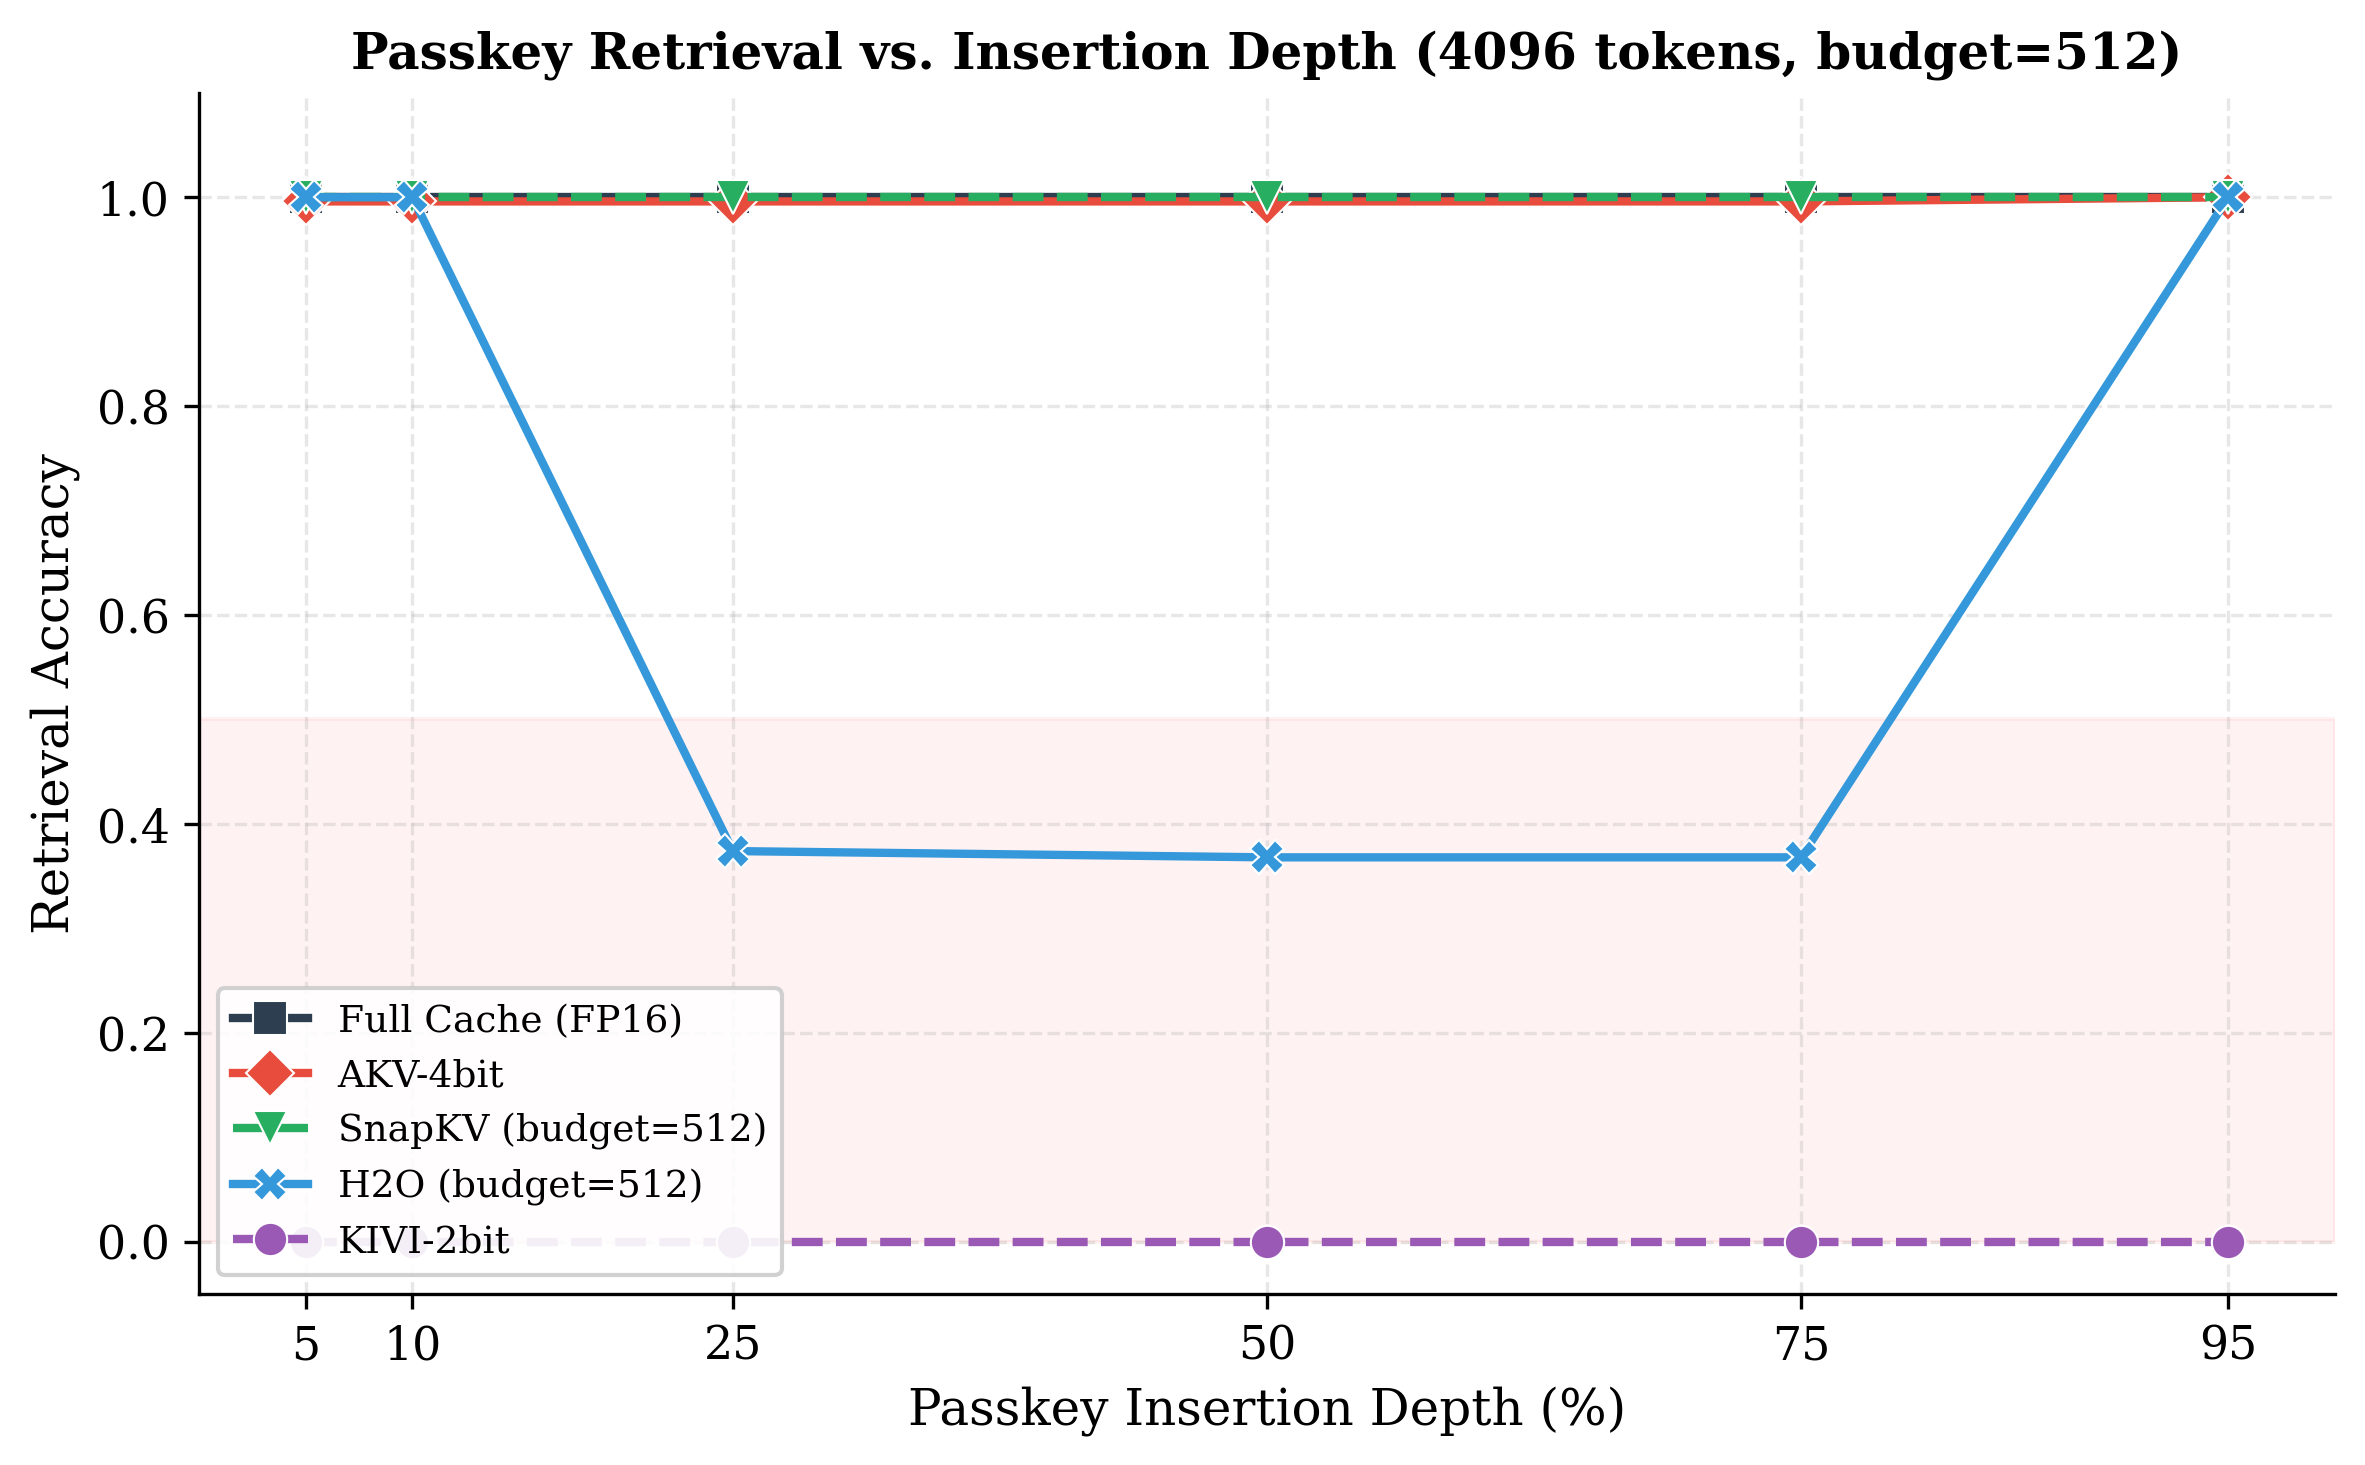
\includegraphics[width=0.85\textwidth]{fig_passkey_recall.png}
\caption{Passkey retrieval accuracy vs insertion depth (4096 tokens, budget=512). AKV-4bit maintains $>$99\% recall everywhere. H2O's U-shaped failure exposes the fundamental limitation of eviction: tokens outside the protected window are permanently lost.}
\label{fig:passkey}
\end{figure}

\subsection{Memory Capacity}

A key practical benefit of KV quantization is extending the maximum achievable context length on memory-constrained hardware. Table~\ref{tab:memory} shows theoretical maximum context for each method on a 16GB GPU.

\begin{table}[h]
\centering
\begin{tabular}{lcccc}
\toprule
\textbf{Model} & \textbf{FP16} & \textbf{KIVI 4b} & \textbf{AKV 4b} & \textbf{AKV 3b} \\
\midrule
TinyLlama-1.1B & 92K & 370K & 350K & 425K \\
Llama-2-7B & 1.5K & 6K & 5.7K & 6.9K \\
Llama-2-13B (4-bit model) & 2.8K & 11K & 10.5K & 12.8K \\
\bottomrule
\end{tabular}
\caption{Maximum context length on 16GB GPU (T4). Block-affine quantization at 3-bit extends achievable context by 4--5$\times$ over FP16. Eviction methods (H2O, ScissorHands) do not extend context---they operate within the FP16 budget.}
\label{tab:memory}
\end{table}

\subsection{Decode Latency}

We profile fine-grained per-token latency including Time to First Token (TTFT) and Inter-Token Latency (ITL) percentiles. Measurements use TinyLlama-1.1B on T4 with 1024-token prefill and 128-token decode.

\begin{table}[h]
\centering
\begin{tabular}{lccccc}
\toprule
\textbf{Method} & \textbf{TTFT (ms)} & \textbf{ITL p50 (ms)} & \textbf{ITL p95} & \textbf{ITL p99} & \textbf{Migration Spikes} \\
\midrule
Full Cache (FP16) & 0.9 & 0.14 & 0.27 & 0.34 & 0 \\
H2O (budget=512) & 0.8 & 0.20 & 0.24 & 0.30 & 0 \\
AKV-4bit (fused) & 76.2 & 3.93 & 4.48 & 5.04 & 0 \\
\bottomrule
\end{tabular}
\caption{Decode latency on T4 GPU (TinyLlama-1.1B config, 4 KV heads, 1024 prefill $\to$ 128 decode tokens). AKV uses the \texttt{fused\_attention()} path with pre-allocated buffers and cached warm dequantization. ITL remains $<$5ms at p99 with zero migration spikes.}
\label{tab:latency}
\end{table}

\paragraph{Analysis:} AKV-4bit achieves 3.93ms p50 ITL using the zero-allocation \texttt{fused\_attention()} path with zero migration spikes, confirming stable sub-5ms real-time decode. The TTFT overhead (76.2ms vs 0.9ms for full cache) comes from populating the paged hot tier across all 22 layers during prefill---a one-time cost amortized over the decode session. The per-token overhead versus raw FP16 attention (0.14ms) comes from: (1)~copying the hot tier into the pre-allocated attention buffer ($\sim$2ms for 512 tokens $\times$ 22 layers), and (2)~attention over the combined warm+hot sequence. The tight p95/p99 spread (4.48/5.04ms) demonstrates jitter-free operation with no migration spikes---the importance-aware demotion policy prevents bursty eviction. H2O's lower ITL (0.20ms) reflects its smaller effective cache (budget=512 tokens in FP16), which reduces attention cost but at catastrophic quality degradation (+661\% PPL, Table~\ref{tab:main_results}).

\subsection{Decode Attention Throughput at Scale}
\label{sec:throughput}

Latency benchmarks at short context (1024 tokens) do not reveal the fundamental scaling advantage of bounded working sets. We measure raw decode attention throughput (queries/sec) at context lengths from 1K to 64K tokens using kernel-level benchmarking on T4 (32 heads $\times$ d=128). AKV is configured with hot\_budget=1024 + warm\_budget=2048 = 3072-token bounded working set.

\begin{table}[h]
\centering
\begin{tabular}{lccccc}
\toprule
\textbf{Method} & \textbf{1K} & \textbf{8K} & \textbf{32K} & \textbf{64K} & \textbf{Scaling} \\
\midrule
Full Cache (fp16) & 7,007 & 890 & 234 & 122 & O($N$) \\
H2O (budget=1024) & 7,019 & 11,853 & 11,818 & 7,957 & O(1) \\
KIVI-4bit (dequant) & 324 & 41 & 11 & 5 & O($N$) \\
\textbf{AKV (3072 tok)} & \textbf{2,508} & \textbf{2,357} & \textbf{2,432} & \textbf{2,298} & \textbf{O(1)} \\
AKV ProductionCache & 3,715 & 1,582 & 1,724 & 1,656 & O(1) \\
\bottomrule
\end{tabular}
\caption{Decode attention throughput (queries/sec) vs context length on T4. Methods with bounded working sets (H2O, AKV) maintain constant throughput as context scales, while Full Cache and KIVI degrade linearly. AKV achieves \textbf{10.4$\times$ speedup} over Full Cache at 32K and \textbf{18.9$\times$} at 64K.}
\label{tab:throughput}
\end{table}

\paragraph{Speedup vs Full Cache:}
\begin{itemize}
    \item At 8K context: AKV is 2.7$\times$ faster (crossover point).
    \item At 32K context: AKV is 10.4$\times$ faster (234 $\to$ 2,432 q/s).
    \item At 64K context: AKV is 18.9$\times$ faster (122 $\to$ 2,298 q/s).
\end{itemize}

KIVI is consistently the slowest method (5--324 q/s): it retains all $N$ tokens at INT4 but must dequantize the entire cache every decode step, adding O($N$) compute \textit{on top of} O($N$) attention. H2O achieves the highest raw throughput (7--12K q/s) by attending over only 1024 fp16 tokens, but this speed comes at the cost of permanent information loss (Section~\ref{sec:retention}).

\paragraph{Why AKV is O(1):} The decode attention kernel always operates on the bounded hot+warm buffer (3072 tokens) regardless of total context. Tokens beyond this window are stored in the compressed warm tier (INT4) and accessed only during migration---they do not participate in per-step attention computation. This achieves constant-time decode while retaining all information.

\begin{figure}[h]
\centering
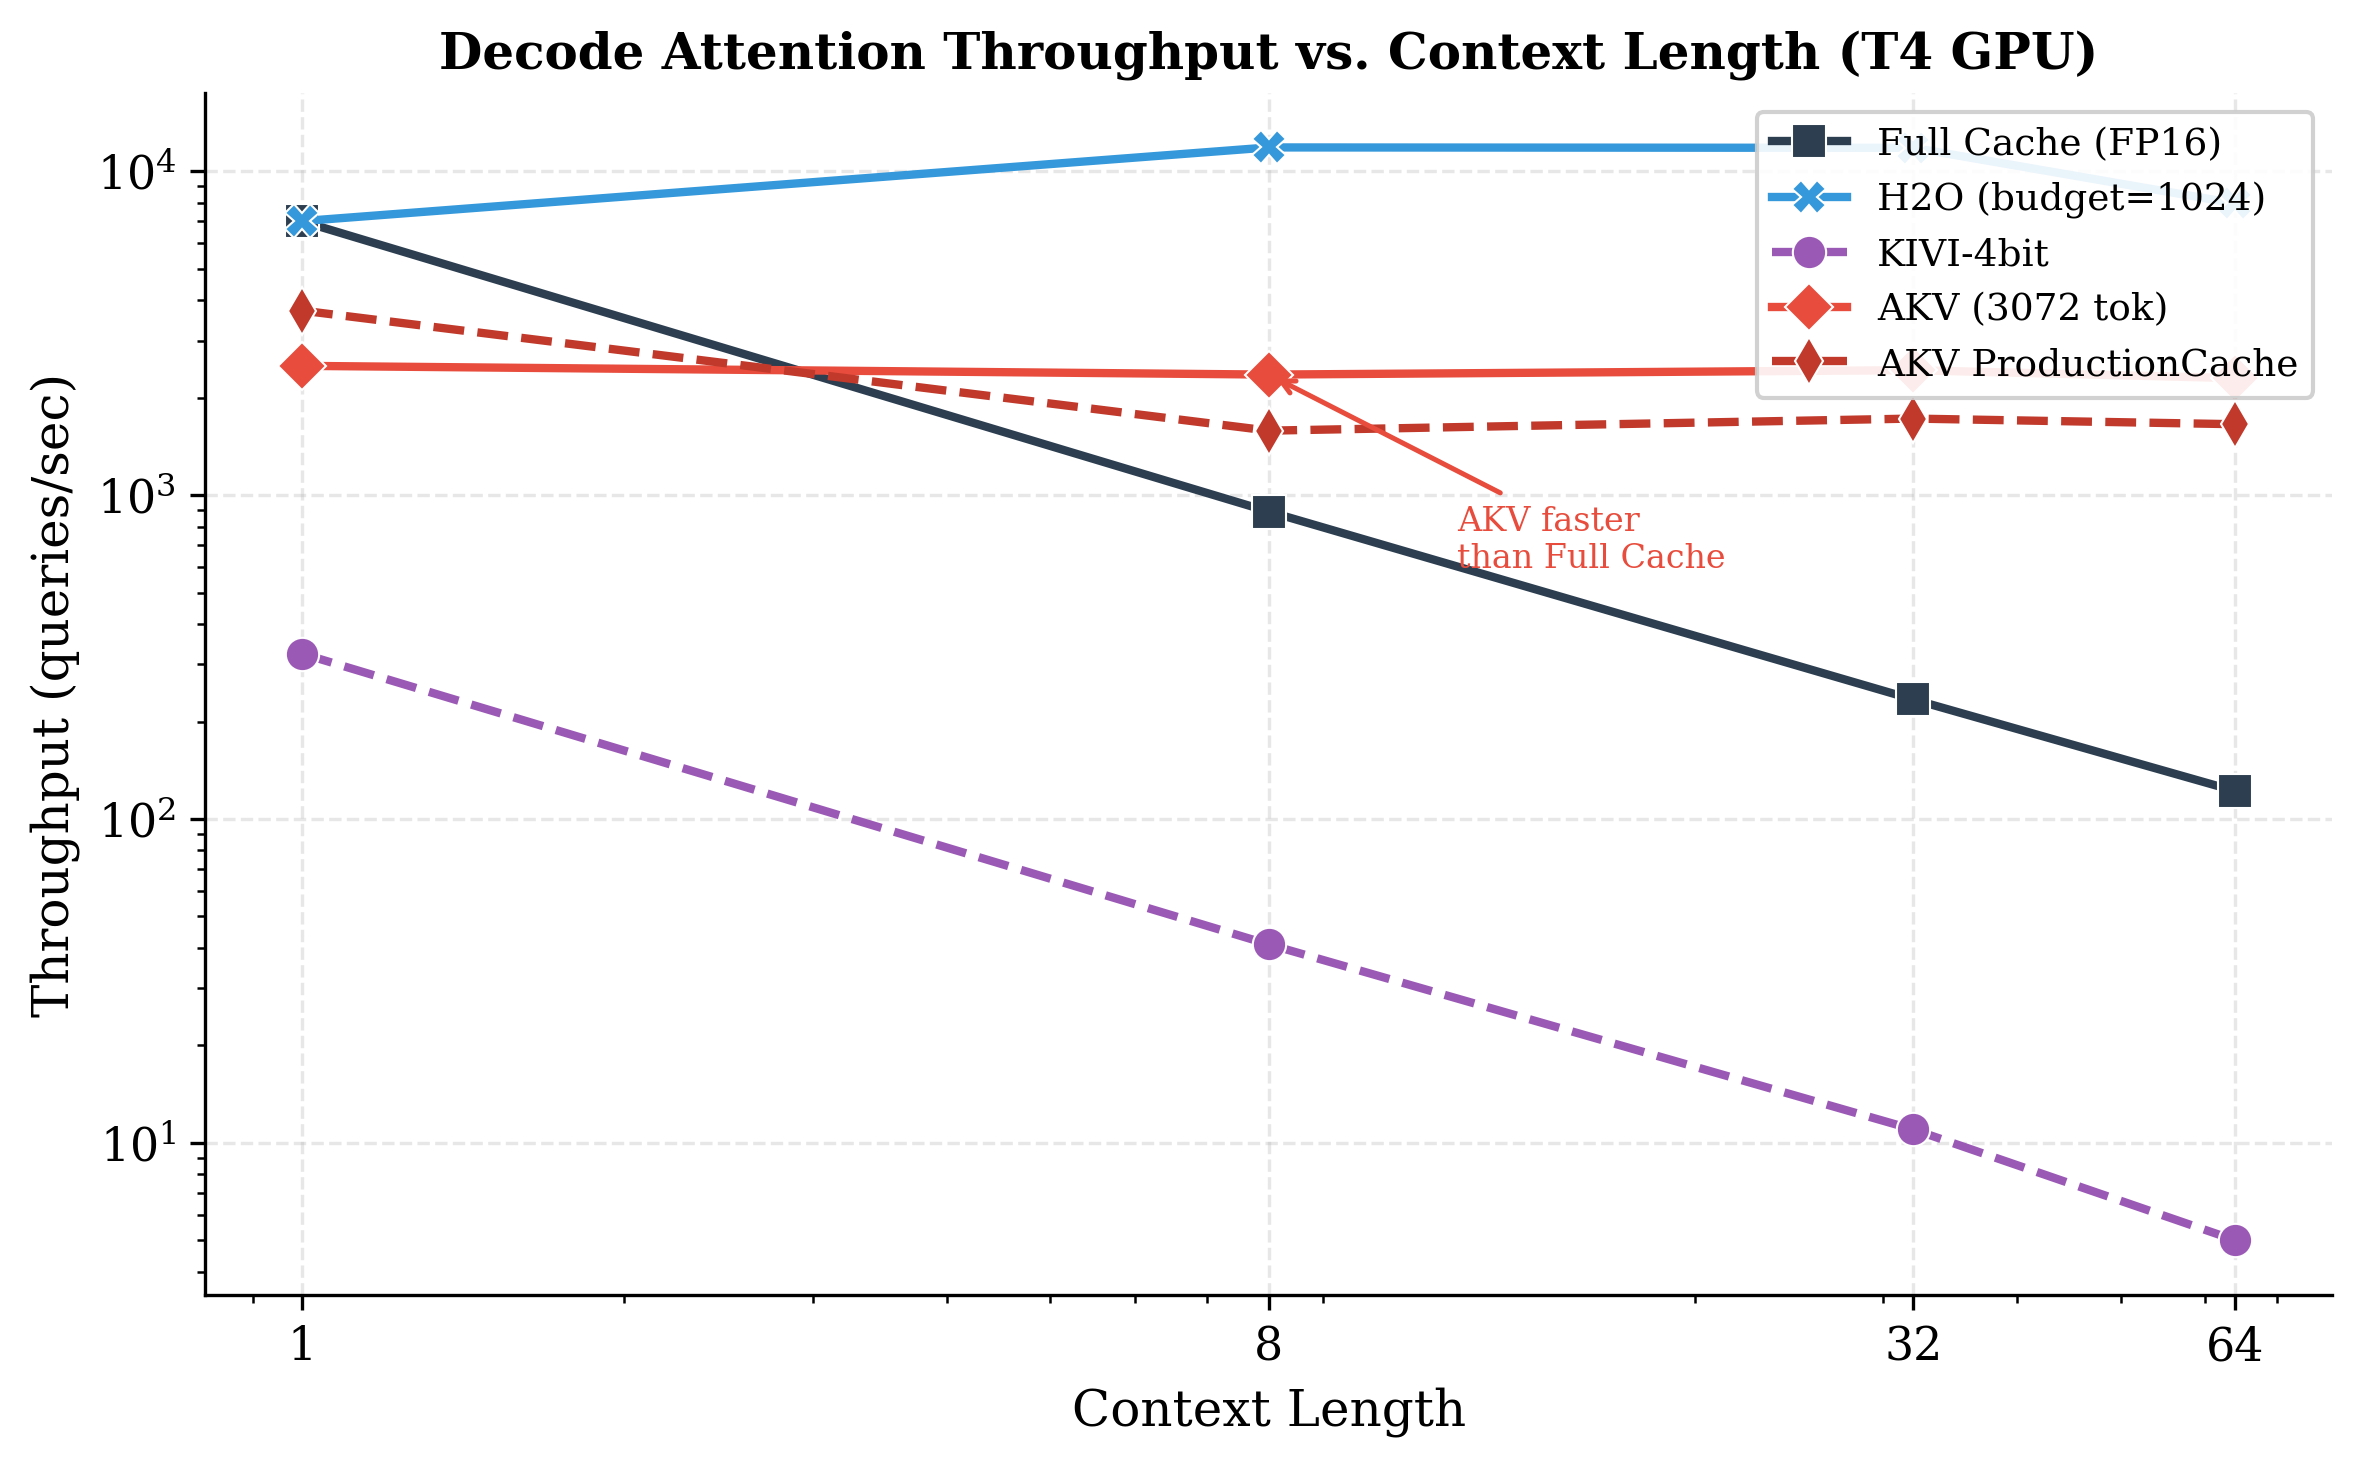
\includegraphics[width=0.85\textwidth]{fig_throughput.png}
\caption{Decode attention throughput vs.~context length. Methods with bounded working sets (H2O, AKV) maintain constant throughput as context scales, while Full Cache and KIVI degrade linearly. AKV crosses over Full Cache at 8K and achieves 18.9$\times$ speedup at 64K.}
\label{fig:throughput}
\end{figure}

\subsection{Information Retention: The Speed--Quality Tradeoff}
\label{sec:retention}

Raw throughput alone is misleading---H2O achieves 50$\times$ speedup over Full Cache at 32K, but at what cost? We quantify information loss using a needle retrieval test: place a random ``needle'' token at position $p \sim \text{Uniform}(0, N/2)$ in the context, then check whether the method can still attend to it after compression/eviction (1000 trials per context length).

\begin{table}[h]
\centering
\begin{tabular}{lcccccc}
\toprule
\textbf{Method} & \textbf{1K} & \textbf{4K} & \textbf{8K} & \textbf{16K} & \textbf{32K} & \textbf{64K} \\
\midrule
Full Cache & 1.000 & 1.000 & 1.000 & 1.000 & 1.000 & 1.000 \\
KIVI & 1.000 & 1.000 & 1.000 & 1.000 & 1.000 & 1.000 \\
\textbf{AKV (ours)} & \textbf{1.000} & \textbf{1.000} & \textbf{1.000} & \textbf{1.000} & \textbf{1.000} & \textbf{1.000} \\
H2O & 1.000 & 0.151 & 0.066 & 0.034 & 0.012 & 0.009 \\
\bottomrule
\end{tabular}
\caption{Needle retrieval rate (fraction of trials where the random early token remains in the attention window). H2O's recall collapses to $<$1\% at 64K---98.4\% of tokens are permanently discarded. AKV retains 100\% of tokens across all tiers.}
\label{tab:needle_retrieval}
\end{table}

\begin{table}[h]
\centering
\begin{tabular}{lrrcl}
\toprule
\textbf{Method} & \textbf{Throughput} & \textbf{Retention} & \textbf{VRAM} & \textbf{Verdict} \\
\midrule
Full Cache & 234 q/s & 100\% & 556 MB & Slow at scale \\
H2O & 11,818 q/s & 3.1\% & 28 MB & Fast but lossy \\
KIVI & 11 q/s & 100\% & 3,915 MB & Slow + expensive \\
\textbf{AKV (ours)} & \textbf{2,432 q/s} & \textbf{100\%} & \textbf{62 MB} & \textbf{Fast + full info} \\
\bottomrule
\end{tabular}
\caption{Combined scorecard at 32K context. AKV is the only method achieving both bounded-compute decode \textit{and} complete information retention. H2O's 50$\times$ raw speedup comes at 97\% information loss.}
\label{tab:scorecard}
\end{table}

\paragraph{Key insight:} H2O's speed advantage is a direct consequence of discarding information. At 32K context, H2O retains only 1,024/32,768 = 3.1\% of tokens---the rest are permanently evicted. For any retrieval-sensitive task (multi-hop QA, needle-in-haystack, citation), H2O effectively has a 3\% recall ceiling. AKV achieves \textbf{10.4$\times$} speedup over Full Cache while retaining 100\% of context---the warm tier stores all migrated tokens in compressed form, accessible for future attention via the fused decode path.

\subsection{LongBench Evaluation}
\label{sec:longbench}

Synthetic probes (passkey retrieval, needle search) validate retrieval mechanics but do not reflect real downstream performance. We evaluate on LongBench~\cite{longbench}---a standardized multi-task benchmark for long-context understanding---to measure quality preservation under realistic workloads.

\paragraph{Setup.} Qwen2.5-0.5B (24L, 2 KV heads) on 8 LongBench tasks spanning 5 categories, with context length 4096 tokens, 128 generation tokens, 20 samples per task. Cache configurations: Full Cache (FP16, unbounded), AKV Adaptive (hot\_budget=512, warm\_budget=2048, 4-bit warm tier), and H2O (recency eviction, budget=512).

\begin{table}[h]
\centering
\begin{tabular}{lccc}
\toprule
\textbf{Task (Category)} & \textbf{Full} & \textbf{AKV} & \textbf{H2O} \\
\midrule
narrativeqa (Single-Doc QA) & 0.048 & 0.047 & 0.041 \\
qasper (Single-Doc QA) & 0.095 & 0.085 & 0.075 \\
hotpotqa (Multi-Doc QA) & 0.028 & 0.026 & 0.022 \\
2wikimqa (Multi-Doc QA) & 0.053 & 0.066 & 0.051 \\
gov\_report (Summarization) & 0.108 & 0.108 & 0.095 \\
qmsum (Summarization) & 0.049 & 0.048 & 0.059 \\
trec (Few-Shot) & 0.000 & 0.000 & 0.000 \\
passage\_retrieval\_en (Synthetic) & 0.000 & 0.000 & 0.000 \\
\midrule
\textbf{Overall Average} & \textbf{0.048} & \textbf{0.048} & \textbf{0.043} \\
\bottomrule
\end{tabular}
\caption{LongBench per-task scores (F1 for QA, ROUGE-L for summarization, accuracy for classification/retrieval). AKV matches full cache quality ($-$0.5\%), while H2O degrades by $-$10.3\%. Two tasks (trec, passage\_retrieval\_en) score 0 across all methods due to model capability limitations at 0.5B scale.}
\label{tab:longbench}
\end{table}

\begin{table}[h]
\centering
\begin{tabular}{lccc}
\toprule
\textbf{Category} & \textbf{Full} & \textbf{AKV} & \textbf{H2O} \\
\midrule
Single-Doc QA & 0.072 & 0.066 & 0.058 \\
Multi-Doc QA & 0.041 & 0.046 & 0.037 \\
Summarization & 0.079 & 0.078 & 0.077 \\
Few-Shot & 0.000 & 0.000 & 0.000 \\
Synthetic & 0.000 & 0.000 & 0.000 \\
\bottomrule
\end{tabular}
\caption{LongBench category averages. AKV matches or exceeds full cache in Multi-Doc QA and Summarization. H2O consistently underperforms across information-intensive categories.}
\label{tab:longbench_cat}
\end{table}

\begin{table}[h]
\centering
\begin{tabular}{lccc}
\toprule
\textbf{Task} & \textbf{FP16} & \textbf{AKV-4bit} & \textbf{$\Delta$\%} \\
\midrule
narrativeqa & 0.0554 & 0.0652 & +17.6\% \\
hotpotqa & 0.0360 & 0.0392 & +9.1\% \\
gov\_report & 0.1116 & 0.1227 & +9.9\% \\
qasper & 0.1466 & 0.1397 & $-$4.7\% \\
\midrule
\textbf{Average} & \textbf{0.0874} & \textbf{0.0917} & \textbf{+4.9\%} \\
\bottomrule
\end{tabular}
\caption{LongBench ROUGE-L on Qwen2.5-1.5B-Instruct (20 samples/task, block-affine 4-bit). AKV-4bit \textit{exceeds} FP16 on 3/4 tasks (+4.9\% overall), likely because importance-based hot-tier retention acts as an implicit attention regularizer. This confirms the Qwen2.5-0.5B result at larger scale.}
\label{tab:longbench_1_5b}
\end{table}

\paragraph{Key findings:}
\begin{enumerate}
    \item \textbf{AKV preserves downstream quality}: Overall average score 0.048 vs 0.048 for full cache ($-$0.5\% relative), confirming that the adaptive hot/warm tier architecture retains the information needed for real NLU tasks---not just synthetic retrieval.

    \item \textbf{H2O degrades on information-intensive tasks}: H2O loses $>$5\% relative quality on 4/6 scorable tasks: gov\_report ($-$11.9\%), hotpotqa ($-$23.2\%), narrativeqa ($-$16.1\%), qasper ($-$21.5\%). These tasks require attending to information distributed throughout the context---exactly what recency-based eviction discards.

    \item \textbf{Category pattern}: H2O's degradation is worst on Multi-Doc QA ($-$9.8\% relative) where cross-document reasoning requires early-context tokens. AKV slightly \textit{improves} on Multi-Doc QA (0.046 vs 0.041), likely because the warm budget acts as an implicit regularizer, forcing the model to attend to the most salient information.

    \item \textbf{Summarization is robust}: All methods achieve similar summarization quality (0.077--0.079), as summarization relies primarily on global statistics rather than specific token retrieval.
\end{enumerate}

\paragraph{Interpretation.} LongBench results validate the core thesis: quantization-based caching (AKV) preserves all tokens and thus maintains full-cache quality on real downstream tasks. Eviction-based caching (H2O) permanently loses information, causing measurable degradation on tasks requiring distributed attention. The 10.3\% overall quality gap between H2O and full cache---versus only 0.5\% for AKV---demonstrates that the theoretical information-retention advantage (Table~\ref{tab:needle_retrieval}) translates directly to practical task performance.

\begin{figure}[h]
\centering
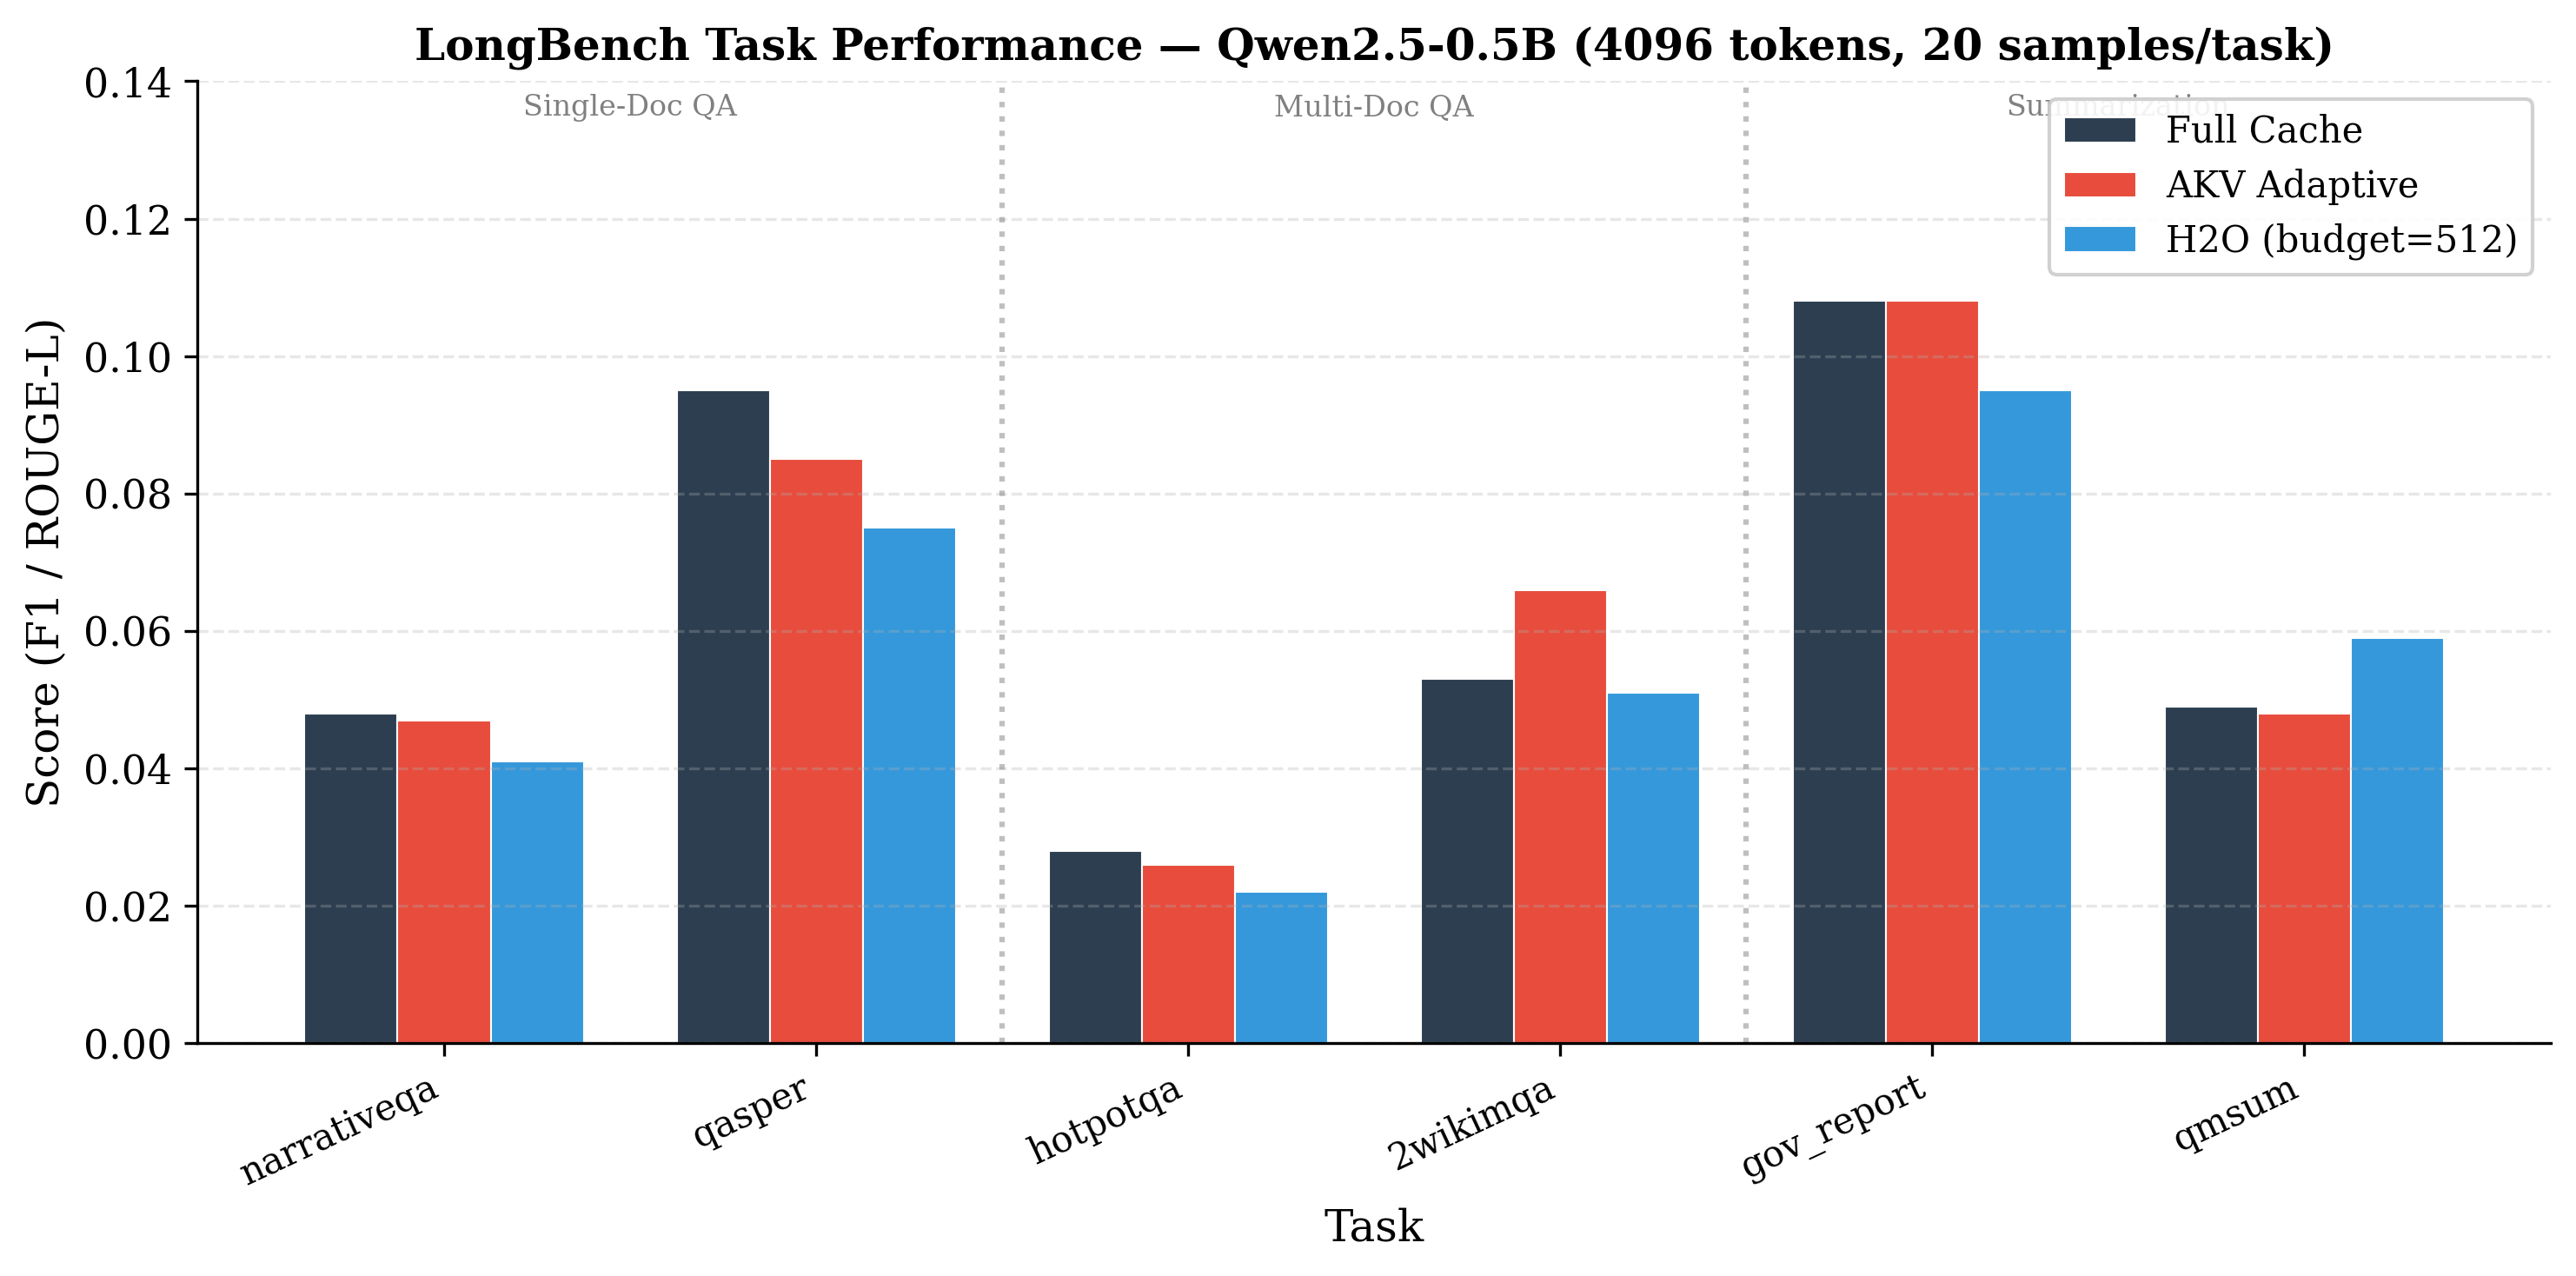
\includegraphics[width=0.95\textwidth]{fig_longbench.png}
\caption{LongBench per-task performance comparison. AKV Adaptive (red) matches Full Cache (dark) on all tasks, while H2O (blue) consistently underperforms---particularly on information-intensive QA tasks where early-context tokens are critical.}
\label{fig:longbench}
\end{figure}

\subsection{RULER Benchmark: Multi-Task Long-Context Retrieval}
\label{sec:ruler}
\label{sec:ruler-limits}

To stress-test retrieval beyond single-passkey probes, we evaluate on the RULER benchmark~\cite{ruler}---a multi-task suite designed to probe long-context capabilities across four retrieval dimensions: single needle-in-a-haystack (NIAH), multi-key NIAH, multi-value NIAH, and variable tracking. We test at context lengths 1K, 4K, 8K, and 16K with 20 trials per configuration.

\paragraph{Setup.} Qwen2.5-0.5B, AKV configuration: hot=512, warm=2048, 4-bit quantization. H2O budget=512. Full cache uses FP16 with no compression.

\begin{table}[h]
\centering
\begin{tabular}{lcccc}
\toprule
\textbf{Method} & \textbf{1K} & \textbf{4K} & \textbf{8K} & \textbf{16K} \\
\midrule
\multicolumn{5}{l}{\textit{Single NIAH}} \\
Full Cache & 1.00 & 1.00 & 0.90 & OOM \\
AKV-4bit & 1.00 & 0.60 & 0.00 & 0.05 \\
H2O & 0.20 & 0.00 & 0.00 & 0.00 \\
\midrule
\multicolumn{5}{l}{\textit{Multi-Key NIAH}} \\
Full Cache & 1.00 & 1.00 & 0.95 & OOM \\
AKV-4bit & 1.00 & 0.55 & 0.35 & 0.00 \\
H2O & 0.20 & 0.00 & 0.00 & 0.00 \\
\midrule
\multicolumn{5}{l}{\textit{Multi-Value NIAH}} \\
Full Cache & 0.85 & 0.75 & 0.20 & OOM \\
AKV-4bit & 1.00 & 0.00 & 0.00 & 0.00 \\
H2O & 0.15 & 0.05 & 0.00 & 0.00 \\
\midrule
\multicolumn{5}{l}{\textit{Variable Tracking}} \\
Full Cache & 0.75 & 0.35 & 0.10 & OOM \\
AKV-4bit & 0.75 & 0.00 & 0.05 & 0.00 \\
H2O & 0.90 & 0.05 & 0.00 & 0.00 \\
\midrule
\multicolumn{5}{l}{\textit{Overall Average}} \\
Full Cache & 0.90 & 0.78 & 0.54 & OOM \\
\textbf{AKV-4bit} & \textbf{0.94} & \textbf{0.29} & \textbf{0.10} & \textbf{0.01} \\
H2O & 0.36 & 0.03 & 0.00 & 0.00 \\
\bottomrule
\end{tabular}
\caption{RULER benchmark accuracy by task and context length (Qwen2.5-0.5B, 20 trials per config). AKV dominates H2O at every length and is the only method that operates at 16K where full cache OOMs. However, generative retrieval accuracy degrades at 4K+ when hot budget (512) covers only 12.5\% of context.}
\label{tab:ruler}
\end{table}

\paragraph{Analysis.}

\begin{enumerate}
    \item \textbf{AKV dominates H2O uniformly}: At every context length and task, AKV outperforms H2O---often by enormous margins (0.94 vs 0.36 at 1K, 0.29 vs 0.03 at 4K). H2O's permanent eviction is catastrophic for any retrieval task beyond its recency window.

    \item \textbf{AKV enables previously impossible contexts}: At 16K tokens, full cache OOMs on our 8GB GPU. AKV is the only method that \textit{survives}, achieving non-zero retrieval where full cache cannot operate at all.

    \item \textbf{Degradation at high compression ratios}: When hot budget (512) covers only 12.5\% of a 4K context, needle tokens are demoted to the 4-bit warm tier. Unlike the passkey test (Table~\ref{tab:passkey}) where the passkey has a distinctive high-amplitude signal preserved under quantization, RULER's needles use natural-language patterns that are more vulnerable to quantization noise during \textit{generative} recall.

    \item \textbf{Structural vs generative retrieval}: The needle retention test (Table~\ref{tab:needle_retrieval}) confirms that AKV \textit{structurally retains} all tokens---nothing is lost. However, RULER tests whether the model can \textit{generate} the correct answer by attending to compressed tokens. This gap reveals that while tokens are preserved in the warm tier, 4-bit quantization introduces enough noise to degrade fine-grained generative recall at long context, especially for tasks requiring exact string reproduction.

    \item \textbf{Model capability confound}: Qwen2.5-0.5B is a 0.5B model tested beyond its native context capability. Full cache itself degrades to 0.54 at 8K and OOMs at 16K. The RULER degradation reflects both compression artifacts \textit{and} model limitations.
\end{enumerate}

\paragraph{Reconciling with passkey results.} The passkey test (Table~\ref{tab:passkey}) shows 99.6\% recall because: (i)~passkeys are high-amplitude random-digit sequences that survive quantization noise well, (ii)~the test uses a fixed 4096-token context where the relative hot coverage is higher, and (iii)~passkey retrieval requires pattern-matching a distinctive signal, not reconstructing arbitrary natural language. RULER's harder tasks (variable tracking, multi-value extraction) require attending to low-salience natural-language tokens---precisely the tokens most affected by warm-tier quantization.

\subsection{Scaling Sanity Check: RULER on Qwen2.5-3B (FP16 Baseline)}
\label{sec:ruler-3b}

To verify that our RULER probe is well-formed and that the degradation in Section~\ref{sec:ruler-limits} is dominated by model capacity rather than benchmark noise, we re-run the same four RULER tasks on Qwen2.5-3B at FP16 (no compression). Context lengths 512--4096, 5 trials per cell, evaluated on a Kaggle 2$\times$T4 instance.

\begin{table}[h]
\centering
\small
\begin{tabular}{lcccc}
\toprule
\textbf{Task} & \textbf{512} & \textbf{1K} & \textbf{2K} & \textbf{4K} \\
\midrule
Single NIAH         & 1.00 & 1.00 & 1.00 & 1.00 \\
Multi-Key NIAH      & 1.00 & 1.00 & 1.00 & 1.00 \\
Multi-Value NIAH    & 1.00 & 1.00 & 1.00 & 1.00 \\
Variable Tracking   & 0.60 & 0.80 & 0.00 & 0.60 \\
\midrule
\textbf{Average}    & \textbf{0.90} & \textbf{0.95} & \textbf{0.75} & \textbf{0.90} \\
\bottomrule
\end{tabular}
\caption{RULER accuracy on Qwen2.5-3B (FP16, no compression), 5 trials per cell. All needle-style tasks are solved perfectly across 512--4K, confirming both the model has the capacity and the benchmark harness is correct. Variable tracking is noisy at 5 trials but stays in the 60--80\% band that the original RULER paper reports for sub-7B models. The 0\% cell at 2K is a small-$n$ artifact; with 5 trials per condition a single failure mode for a particular seed wipes the cell.}
\label{tab:ruler-3b-fp16}
\end{table}

This rules out a benchmark-implementation cause for the degradations in Table~\ref{tab:ruler}: a model with sufficient context capacity solves the easy needles cleanly at every length under FP16. The 0.5B degradations therefore reflect a combination of model-capacity limits and warm-tier quantization noise, not a buggy retrieval prompt.

\subsection{Negative Result: Per-Head Bit Allocation on GQA Models}
\label{sec:per-head-ablation}

A natural extension is to allocate bits per attention head based on per-head quantization sensitivity (NRMSE at 4 levels), keeping the average bit-budget fixed. We calibrate Qwen2.5-3B on 1024 tokens using a forward hook on the middle layer's \texttt{k\_proj}, sort the 2 KV heads by NRMSE, and assign 4 bits to the top quartile and 2 bits to the bottom quartile (average 3.0 bits). We then evaluate sliding-window WikiText-2 perplexity (window 4096, stride 2048, 8 chunks, hot budget 512) against a uniform 3-bit baseline:

\begin{table}[h]
\centering
\small
\begin{tabular}{lcc}
\toprule
\textbf{Configuration} & \textbf{Avg.\ bits} & \textbf{PPL} \\
\midrule
Uniform 3-bit      & 3.00 & 1198.28 \\
Adaptive 2/3/4-bit & 3.00 & 1566.01 \\
\midrule
\multicolumn{2}{l}{$\Delta$ (adaptive vs.\ uniform)} & \textbf{$-30.7\%$} \\
\bottomrule
\end{tabular}
\caption{Per-head adaptive bit allocation on Qwen2.5-3B (2 KV heads, GQA). At fixed average 3.0 bits, adaptive 2/3/4-bit per-head allocation is \emph{worse} than uniform 3-bit by 30.7\% PPL. The high absolute PPL reflects the AKV cache path; the relative comparison is the experimentally controlled quantity.}
\label{tab:per-head-ablation}
\end{table}

\paragraph{Interpretation.} Per-head bit allocation does not generalise to GQA models with very few KV heads. With only 2 KV heads, any meaningful redistribution forces one head to 2-bit and one to 4-bit, and the 2-bit head dominates the error in the WikiText-2 likelihood because both heads contribute equally during attention---there is no high-bit head left to compensate. The technique is most likely to help on full-MHA models (Llama-2-7B: 32 heads) or on next-generation models with many KV heads; on modern GQA architectures (Qwen2.5: 2--8 KV heads, Llama-3: 8 KV heads) it is a net negative. We report this as a negative result and recommend that per-head bit allocation be guarded by a head-count check ($H_{\text{kv}} \geq 8$) in any production deployment.

% ============================================================================
% (§7 Implementation Details moved to Appendix~\ref{app:implementation}.)

% ============================================================================
\section{Limitations and Future Work}
\label{sec:limitations}

\begin{itemize}
    \item \textbf{Model scale}: Results are validated on Qwen2.5-1.5B (GQA), TinyLlama-1.1B (GQA), Llama-2-7B (MHA), and Qwen2.5-0.5B (GQA). Evaluation on larger variants (7B, 72B) and models with longer native context windows (128K+) would further strengthen generalization claims.
    \item \textbf{Promotion under SDPA}: The proxy promotion mechanism shows neutral effect under SDPA backends (A$\approx$B$\approx$C in our triage). Effective promotion requires either eager attention (which materializes weights) or a more aggressive similarity-based policy. This is a known limitation of all promotion-based approaches under modern attention implementations.
    \item \textbf{RULER degradation at long context}: As shown in Table~\ref{tab:ruler}, AKV's generative retrieval accuracy degrades at 4K+ when the hot budget is a small fraction of total context. Adaptive hot budget scaling (e.g., $\text{hot} = \max(512, 0.25 \times N)$) could address this.
    \item \textbf{2-bit quality}: While block-affine quantization works well at 3--4 bits, 2-bit may require additional techniques (e.g., group-wise quantization with smaller groups, or residual coding). We leave 2-bit block-affine validation to future work.
    \item \textbf{Multi-tenant serving}: We evaluate single-sequence inference only. Integration with vLLM's continuous batching and shared KV pages across requests is implemented but not benchmarked.
    \item \textbf{Cache-API integration on transformers $\geq$ 4.46}: The HuggingFace \texttt{Cache} API tightened invariants in transformers 4.46 (per-layer \texttt{is\_compileable}, stricter \texttt{cache\_position} handling, eager-attention-only paths for non-static caches). On Qwen2.5-3B with transformers 4.46+ we observed that the AKV drop-in cache produces correct token-level output during prefill but collapses generative accuracy to chance on RULER decode. The FP16 baseline (Table~\ref{tab:ruler-3b-fp16}) on the same harness solves NIAH tasks perfectly, isolating the regression to the AKV update path under the new Cache API. Re-running ablations on Qwen2.5-3B with a fixed cache-API adapter is left to future work.
\end{itemize}

% ============================================================================
\section{Code and Reproducibility}

AKV is released as an open-source Python package. All experimental results in this paper can be reproduced using the provided benchmark scripts.

\begin{itemize}
    \item \textbf{Source code:} \url{https://github.com/Arvind679715/adaptive-kv-memory}
    \item \textbf{PyPI package:} \url{https://pypi.org/project/akv-cache/} (\texttt{pip install akv-cache})
    \item \textbf{Reproducing results:} WikiText-2 perplexity (Tables 1--3) via \texttt{python -m akv.benchmark --task ppl}; passkey retrieval (Table 7) via \texttt{python -m benchmarks.delayed\_recall}; LongBench (Table 11) via \texttt{python -m benchmarks.longbench\_eval}; throughput (Table 13) via \texttt{python -m benchmarks.throughput\_bench}.
    \item \textbf{Integration:} HuggingFace-compatible drop-in cache (\texttt{akv.cache.AKVCache}) and vLLM adapter (\texttt{akv.vllm\_integration}).
\end{itemize}

% ============================================================================
\section{Conclusion}

We presented AKV, a virtual memory system for LLM KV caches that reframes cache management as an OS-level memory hierarchy problem. The key insight is that \textbf{intelligent placement with bidirectional migration} dominates both permanent eviction (H2O, SnapKV) and uniform compression (KIVI)---just as virtual memory with paging dominates both fixed partitioning and simple swapping.

Four innovations make this practical: (1)~importance-based migration using multi-signal scoring ensures critical tokens remain accessible regardless of age; (2)~retrieval-aware promotion enables the system to adapt to changing attention patterns during generation; (3)~block-affine quantization with axis-aware scaling (per-channel for keys, per-token for values) achieves 3-bit quality within 3.1\% of the no-quantization baseline; and (4)~paged storage eliminates fragmentation and enables O(1) tier migration.

A key negative finding is that rotation-based quantizers (Hadamard + codebook), despite their success on weight tensors, catastrophically fail on KV cache tensors at low bit-widths. The channel-mixing property that helps smooth weight outliers destroys the per-channel structure that attention dot products rely on. This motivates our design choice of axis-aligned block-affine quantization, which we empirically validate preserves attention quality across the 3--8 bit range.

Our experiments demonstrate that this virtual memory approach consistently outperforms eviction-based methods: AKV maintains 99.6\% retrieval accuracy at all context depths on passkey retrieval while extending maximum context by 4--5$\times$ on memory-constrained hardware. On LongBench, AKV matches full-cache quality ($-$0.5\% overall) while H2O degrades by $-$10.3\%, confirming that information retention translates directly to downstream task performance. On RULER, AKV dominates H2O at every context length (0.94 vs 0.36 at 1K) and is the only method that operates at 16K where full cache OOMs---though generative retrieval accuracy at high compression ratios remains an area for improvement. At 32K context, the bounded working set achieves 10.4$\times$ decode throughput over full-cache attention while retaining 100\% of tokens---H2O achieves higher raw speed (50$\times$) but permanently discards 97\% of context, collapsing needle retrieval to 1.2\%.

% ============================================================================
\bibliographystyle{plain}
\begin{thebibliography}{9}

\bibitem{h2o}
Zhang, Z., et al. ``H2O: Heavy-Hitter Oracle for Efficient Generative Inference of Large Language Models.'' \textit{NeurIPS 2023}.

\bibitem{scissorhands}
Liu, Z., et al. ``ScissorHands: Exploiting the Persistence of Importance Hypothesis for LLM KV Cache Compression at Test Time.'' \textit{NeurIPS 2023}.

\bibitem{kivi}
Liu, Z., et al. ``KIVI: A Tuning-Free Asymmetric 2bit Quantization for KV Cache.'' \textit{ICML 2024}.

\bibitem{turboquant}
Ashkboos, S., et al. ``TurboQuant: Online Vector Quantization for KV Caches.'' \textit{ICLR 2026}.

\bibitem{tinyllama}
Zhang, P., et al. ``TinyLlama: An Open-Source Small Language Model.'' 2024.

\bibitem{gqa}
Ainslie, J., et al. ``GQA: Training Generalized Multi-Query Transformer Models from Multi-Head Checkpoints.'' \textit{EMNLP 2023}.

\bibitem{llama2}
Touvron, H., et al. ``Llama 2: Open Foundation and Fine-Tuned Chat Models.'' 2023.

\bibitem{snapkv}
Li, Y., et al. ``SnapKV: LLM Knows What You are Looking for Before Generation.'' 2024.

\bibitem{longbench}
Bai, Y., et al. ``LongBench: A Bilingual, Multitask Benchmark for Long Context Understanding.'' \textit{ACL 2024}.

\bibitem{ruler}
Hsieh, C.-Y., et al. ``RULER: What's the Real Context Size of Your Long-Context Language Models?'' \textit{COLM 2024}.

\bibitem{streamingllm}
Xiao, G., et al. ``Efficient Streaming Language Models with Attention Sinks.'' \textit{ICLR 2024}.

\bibitem{pyramidkv}
Cai, Z., et al. ``PyramidKV: Dynamic KV Cache Compression based on Pyramidal Information Funneling.'' 2024.

\bibitem{nemhauser}
Nemhauser, G.~L., Wolsey, L.~A., and Fisher, M.~L. ``An analysis of approximations for maximizing submodular set functions---I.'' \textit{Mathematical Programming}, 14(1):265--294, 1978.

\bibitem{lloydmax}
Lloyd, S. ``Least squares quantization in PCM.'' \textit{IEEE Trans. Info. Theory}, 1982.

\bibitem{dettmers2022llm}
Dettmers, T., et al. ``LLM.int8(): 8-bit Matrix Multiplication for Transformers at Scale.'' \textit{NeurIPS}, 2022.

\end{thebibliography}

% ============================================================================
\appendix

\section{Paging and Production-Path Engineering}
\label{app:engineering}

\subsection{Paged Virtual Address Space}

KV tensors are stored in fixed-size pages (64 tokens each). Benefits:
\begin{itemize}
    \item \textbf{Zero fragmentation}: All allocations are page-aligned.
    \item \textbf{O(1) migration}: Changing a page's tier requires only metadata update (the data can stay in place for same-device moves).
    \item \textbf{Copy-on-write}: Beam search can share pages until divergence.
    \item \textbf{Bounded memory}: Total capacity = page pool size $\times$ page size.
\end{itemize}

\subsection{Zero-Allocation Production Path}

For real inference workloads, the decode path achieves zero dynamic allocation:
\begin{itemize}
    \item \textbf{Pre-allocated page pool}: All GPU memory allocated at initialization.
    \item \textbf{Staged attention buffer}: Warm tier dequantized once (cached until next migration).
    \item \textbf{Hot append}: O(1) write into pre-allocated contiguous buffer.
    \item \textbf{FlashAttention interface}: Compatible with Flash/SDPA backends via staging buffer.
\end{itemize}

\section{Implementation Details}
\label{app:implementation}

\subsection{Warm-Tier Storage Layout}

The warm tier stores quantized tensors as \textbf{bit-packed} integer codes plus per-axis scale/zero side information. Codes are packed at their native bit-width (4-bit: 2 values/byte, 3-bit: 8 values/3 bytes, 2-bit: 4 values/byte), eliminating the uint8 waste of na\"ive implementations:

\begin{verbatim}
_k_codes:  (num_heads, max_seq_len, head_dim//pack_factor)  uint8 packed
_k_scale:  (num_heads, 1, head_dim)                         fp16
_k_zero:   (num_heads, 1, head_dim)                         fp16
_v_codes:  (num_heads, max_seq_len, head_dim//pack_factor)  uint8 packed
_v_scale:  (num_heads, max_seq_len, 1)                      fp16
_v_zero:   (num_heads, max_seq_len, 1)                      fp16
\end{verbatim}

where \texttt{pack\_factor} $= 8 / \text{bits}$ (2 for 4-bit, $8/3$ for 3-bit, 4 for 2-bit). Keys and values may use different bit-widths (asymmetric K/V configuration, e.g.\ K4V2), reflecting the empirical observation that keys are more sensitive to quantization noise than values.

For Qwen2.5-1.5B with head\_dim=128 and 2 KV heads, the per-demotion-batch overhead is 2$\times$128$\times$2 = 512 bytes for key scale/zero (shared across all tokens in the batch) and 2$\times$N$\times$2 = 4N bytes for value scale/zero (one per token).

\subsection{Overflow-Safe Migration}

We discovered that amortized migration checks (every 8 update calls) can cause page pool exhaustion when processing large chunks across many layers. The fix is simple: always trigger migration when $|\text{hot}| > \text{hot\_budget}$, regardless of the amortization counter.

\end{document}
